\chapter{Methods}
\label{sec:Methods}
Although the particle filter  is a standard Regularized
Particle filter, as described by Arulampalam et al., optimizing the 
particle filter for use with FMRI data is non-trivial \cite{Arulampalam2002a}. 


\section{Model}
As originally written in \autoref{sec:BOLD Physiology} the state variables
for the BOLD model are as follows:
\begin{eqnarray}
\dot{s} &=& \epsilon u(t) - \frac{s}{\tau_s} - \frac{f - 1}{\tau_f} \\
\dot{f} &=& s\\
\dot{v} &=& \frac{1}{\tau_0}(f - v^\alpha)\\
\dot{q} &=& \frac{1}{\tau_0}(\frac{f(1-(1-E_0)^f)}{E_0} - \frac{q}{v^{1-1/\alpha}})
\end{eqnarray}
The original assumption regarding particle filter models (\autoref{sec:Particle Filter Model})
included noise in the update of $x$, however that is not included here.
The reason for the difference is that cloud of particles is, to some extent,
able to account for that noise. It is common, however, to model that noise
in particle filters by adding a random value to each updated state variable. 
Because the purpose of this particle filter is to learn the underlying distribution
of the static parameters, rather than precisely modeling the time course of the 
in the dynamic state variables $\{s,f,v,q\}$ this noise is left out. It also helps
that detrending is applied before the particle filter and that the
BOLD model is dissipative. When no stimuli are applied, all the particles 
decay to ($\{0,1,1,1\}$). Typical particle filters 
also use this state noise as an exploratory measure; however this method is
less necessary when good priors are available.

For all the analyses  in this work, $1400$ integration points
per second were used.  Typically a step size of $0.001$ was sufficient,
however, from time to time $0.001$ can still result in problems for the
BOLD model.

\section{Preprocessing}
\label{sec:Methods Preprocessing}
The normal pipeline for analyzing
FMRI involves a several preprocessing steps. The first and most important
task is motion correction. To do this, a single volume in time is chosen, and
volumes at every other time are realigned to best match the target volume. This corrects
for motion by the patient as well as small changes in the magnetic
fields that cause the image to shift. 
In conventional statistical parametric mapping, a Gaussian smoothing
filter is applied across the image as discussed in \autoref{sec:RFT}.
After this, detrending is performed which is discussed in \autoref{sec:Detrend}.
Recall that FMRI signal levels are unit-less and though detrending is not
always necessary, the data must always be converted 
into \% difference from baseline. 
The generally accepted method is to use a high pass filter, although the
cutoff frequency is application dependent and often applied haphazardly.
Before going into the detrending used in this work, it is necessary to 
discuss the type of noise present in FMRI.

\subsection{BOLD Noise}
\label{sec:Introduction Noise}
As demonstrated in \autoref{sec:BOLD Physiology} the BOLD response has been
extensively studied and despite minor discrepancies, the cause of the BOLD 
signal is well known. However, as FMRI detects an  
aggregate signal over the space of cubic centimeters, there are
plenty of noise sources . Though local neurons act
together (i.e. around the same time), the density of neurons, the
density of capillaries, and slight differences in activation across 
a particular voxel can all lead to signal attenuation and noise. 

A particularly difficult form of noise present in FMRI is a low frequency
drift, often characterized as a Wiener process \cite{Riera2004}. 
Though not present in all regions, as many as ten to fifteen percent
of voxels can be affected \cite{Tanabe2002}, thus it is prevalent enough to cause significant
inference problems \cite{Smith2007}. It is still not
clear what exactly causes this noise, although one possibility is 
the temperature difference in scanner magnetic coils \cite{Smith2007}. 
It is clear that this drift signal is not solely
due to a physiological effects, given its presence in cadavers and phantoms 
\cite{Smith1999}. Interestingly, it is usually spatially correlated, and
more prevalent at interfaces between regions. Though one potential source
could be slight movement, co-registration is standard, making this unlikely. 
Regardless, the problem mandates the use of a high pass filter \cite{Smith2007}.

In order to characterize the noise, I analyzed resting state data.
During resting state, the patient is shown no images, and he is asked
to avoid movement and complex thought.  Overall though there should be 
very little activation, and thus the signal consists entirely of noise. 
Therefore resting state data is perfect for analyzing noise. 
The locations were chosen from points all around the brain, 
all in grey matter voxels. These time
series were chosen because they were representative of different types
of noise found in the resting state data.

The resting state was gathered in the exact same way as the data in 
\autoref{sec:ExperimentConfig}, except without the stimuli.

\begin{figure}
\centering
\subfigure[]{\label{fig:QQDC:A}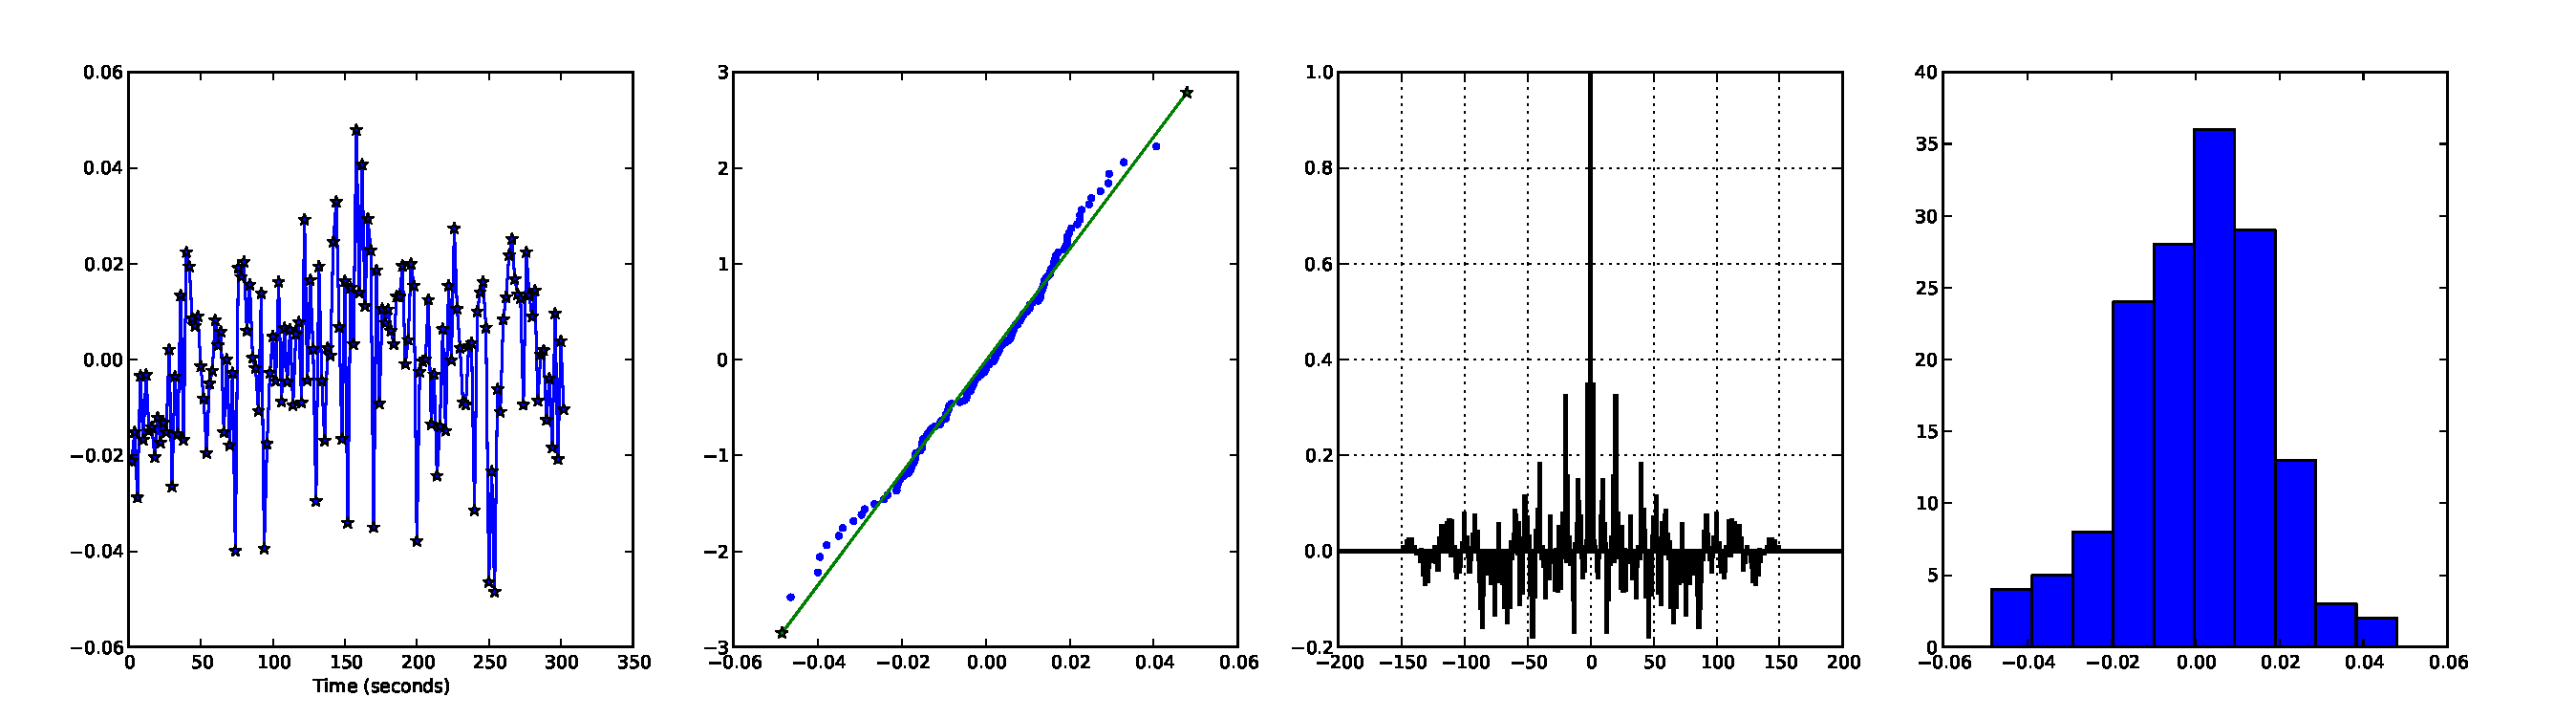
\includegraphics[trim=6cm 1cm 6cm 1cm,width=13cm]{images/noise2_0009_29_49_9}}
\subfigure[]{\label{fig:QQDC:B}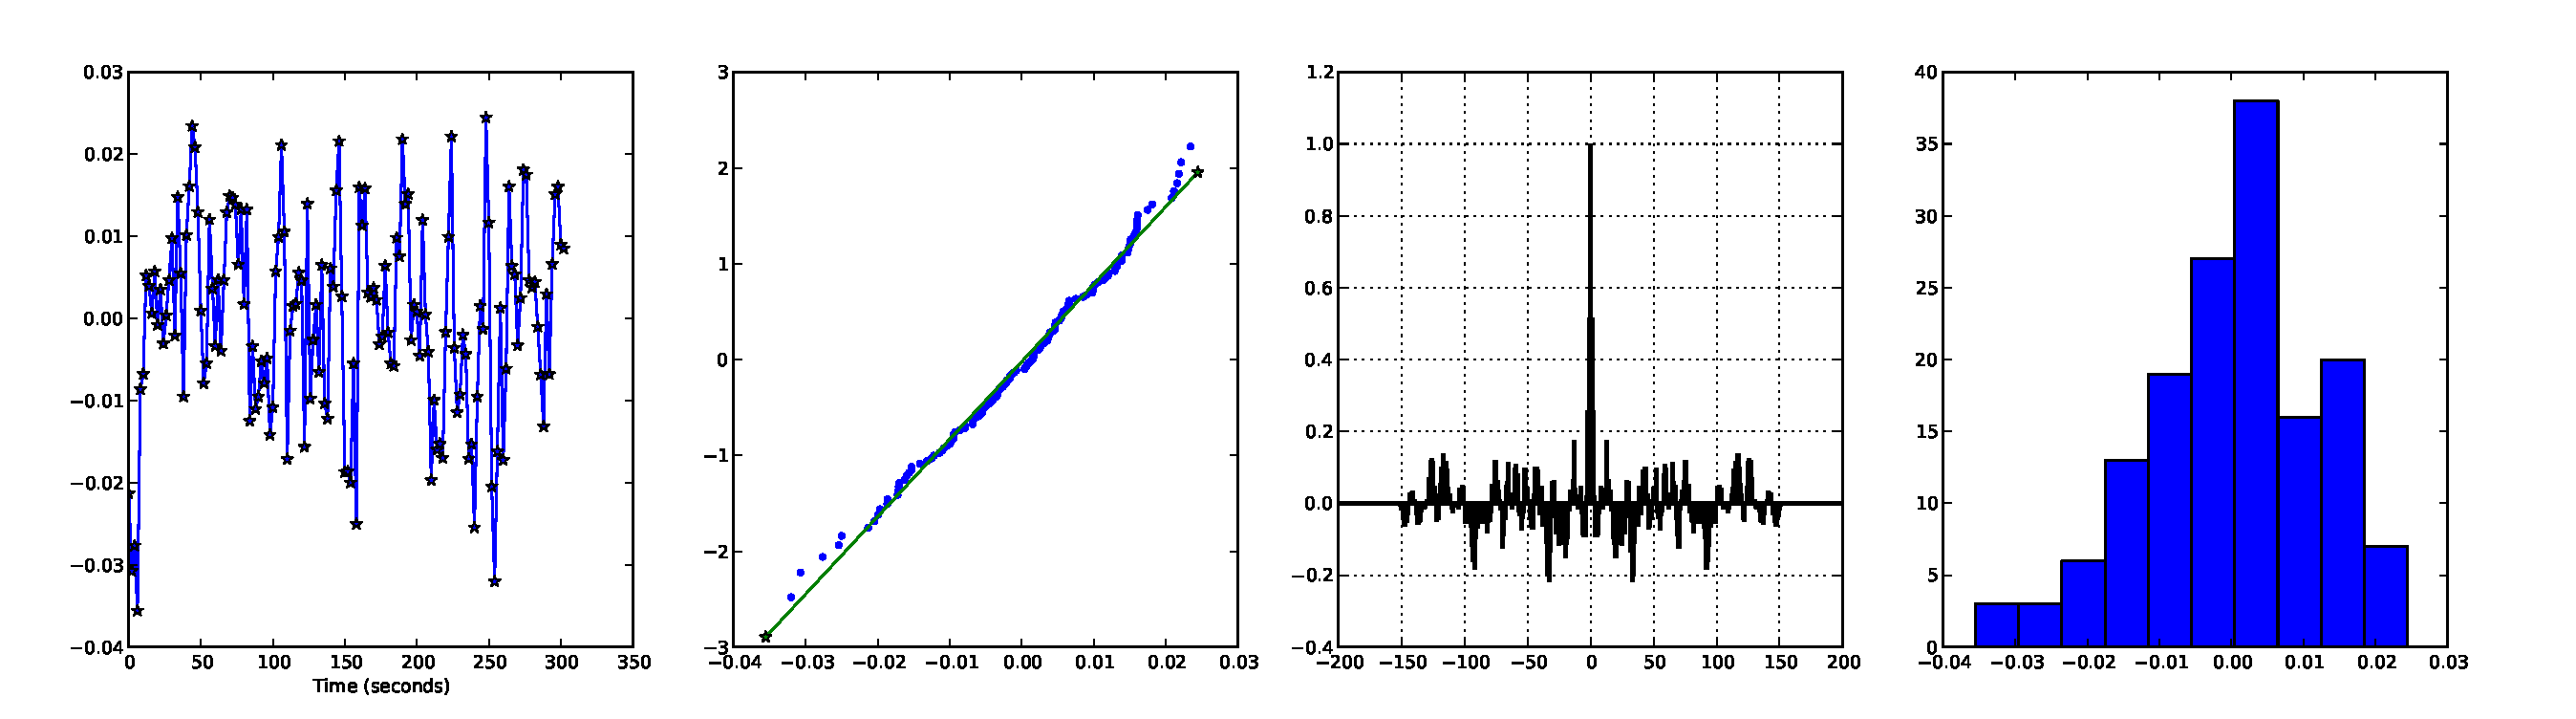
\includegraphics[trim=6cm 1cm 6cm 1cm,width=13cm]{images/noise2_0009_34_43_24}}
\subfigure[]{\label{fig:QQDC:C}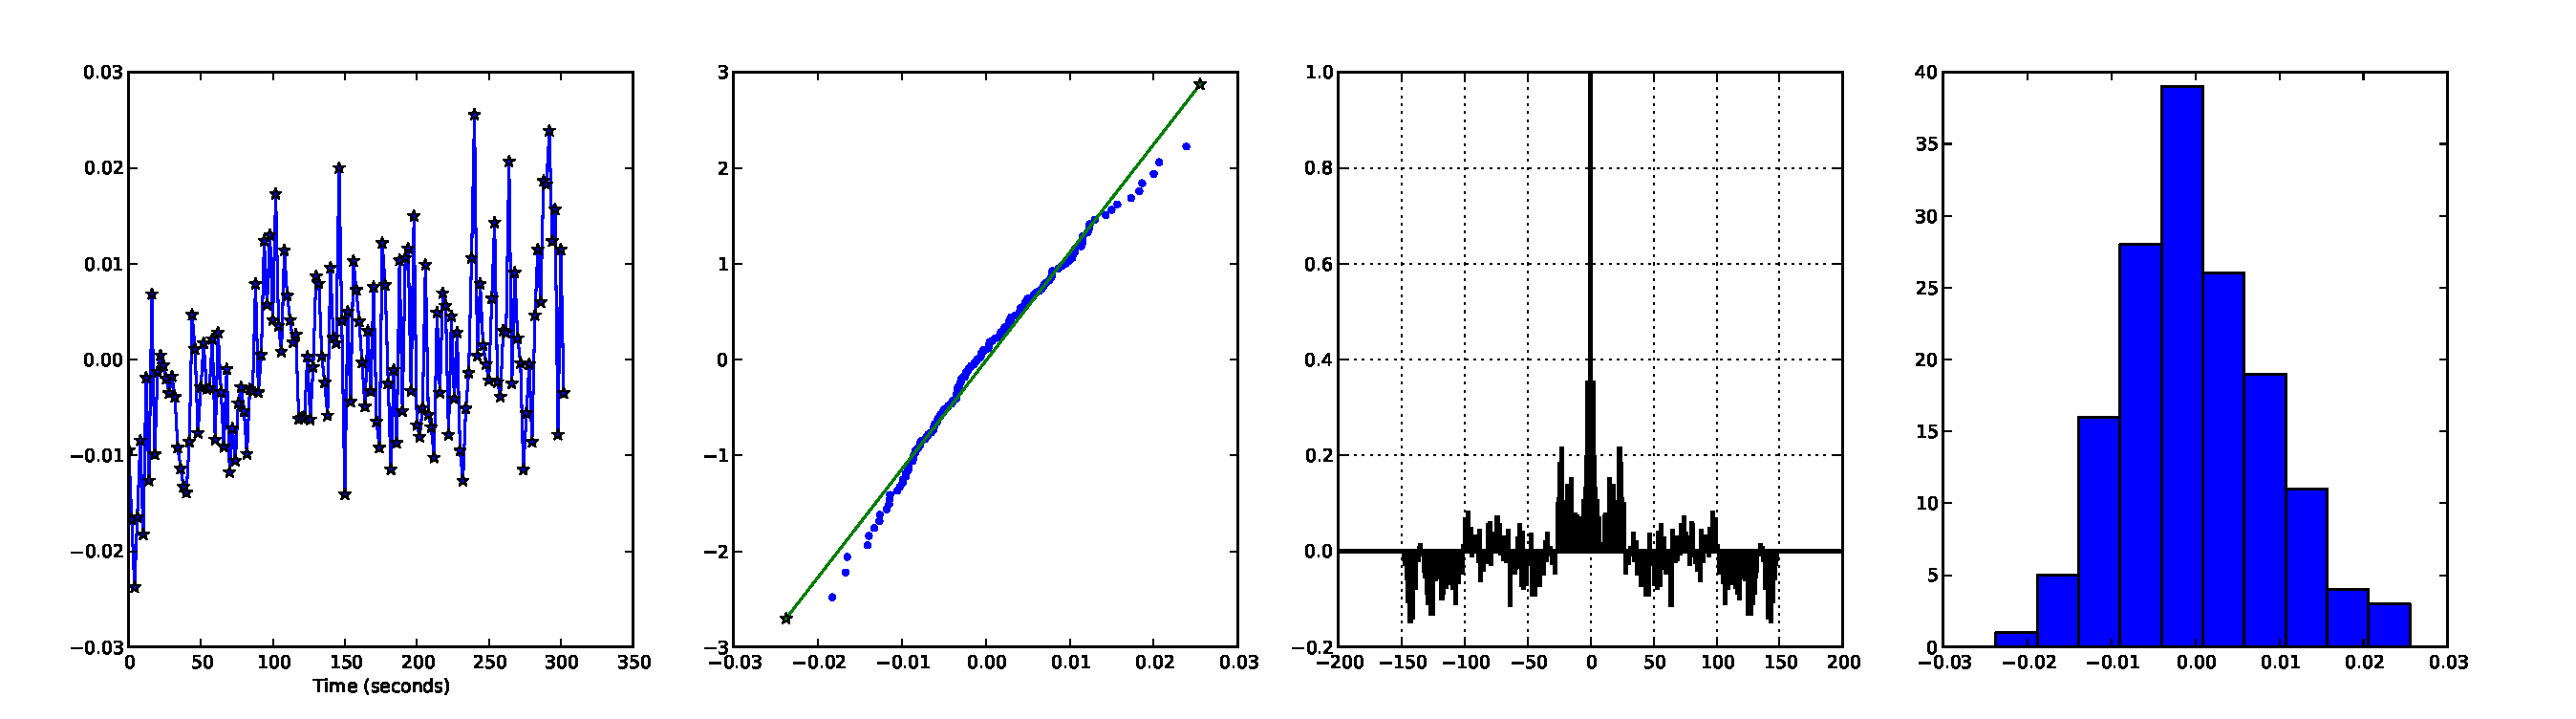
\includegraphics[trim=6cm 1cm 6cm 1cm,width=13cm]{images/noise2_0009_22_38_23}}
\subfigure[]{\label{fig:QQDC:D}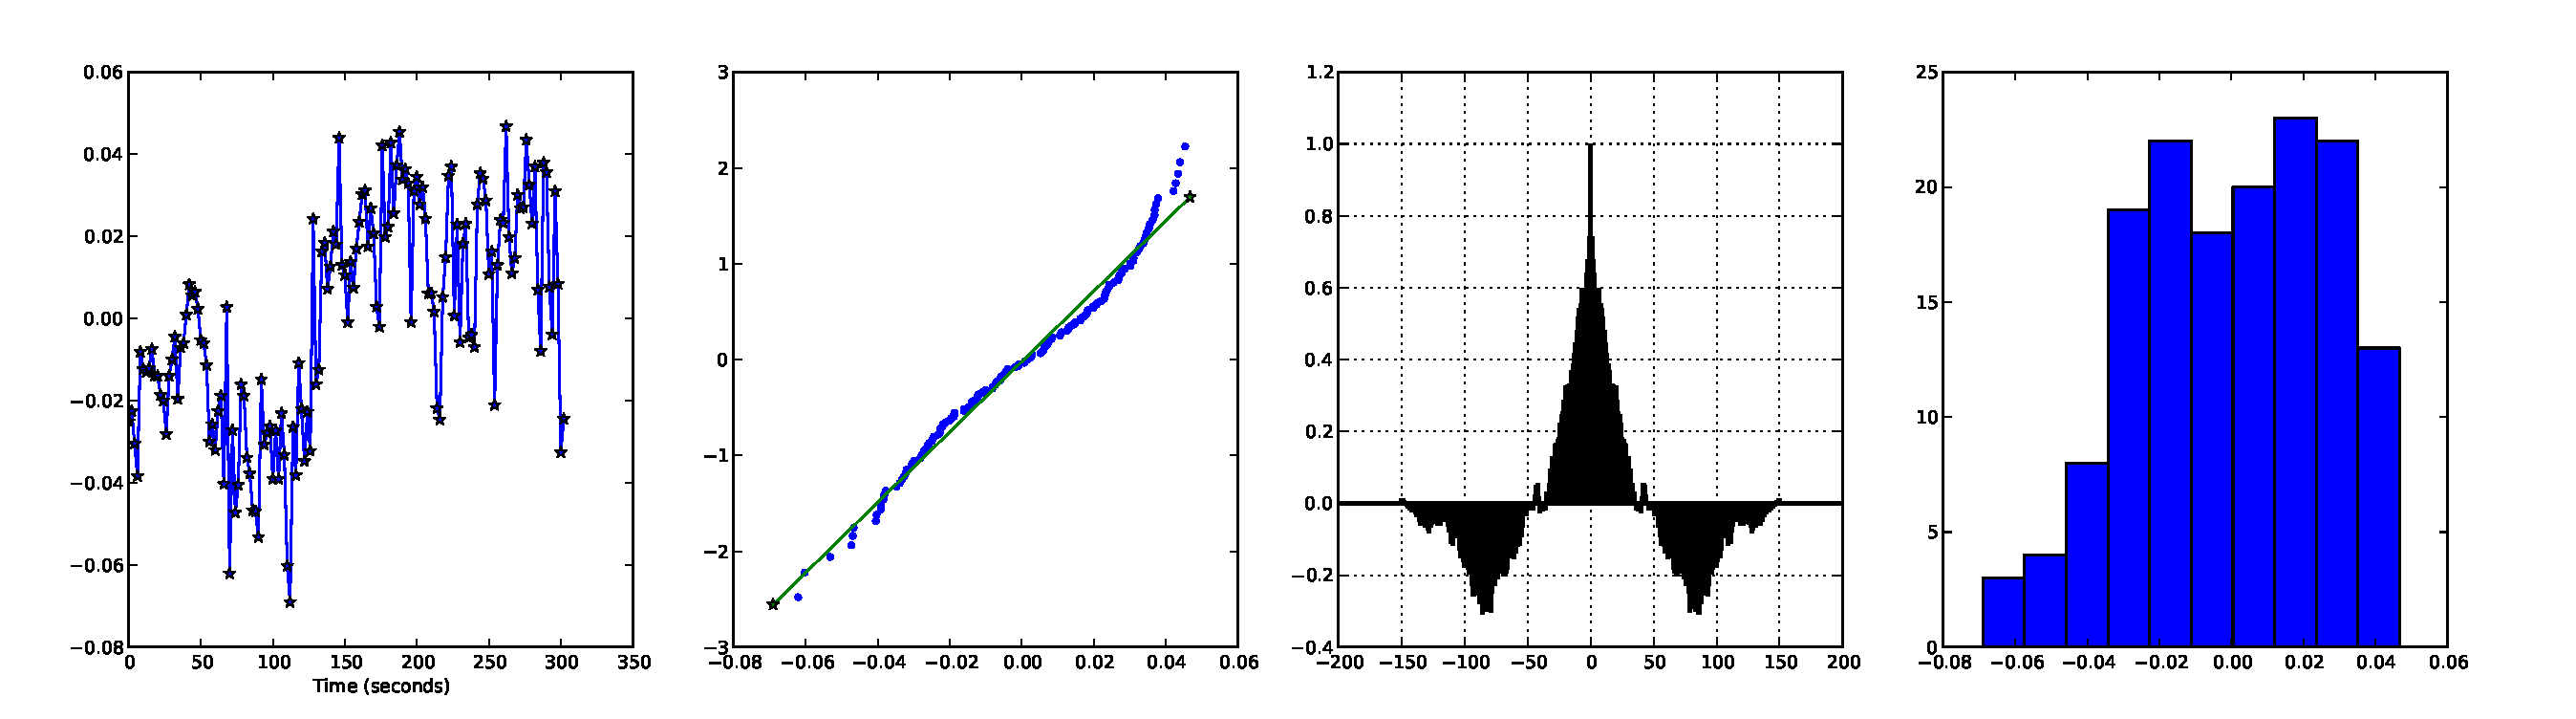
\includegraphics[trim=6cm 1cm 6cm 1cm,width=13cm]{images/noise2_0009_37_29_24}}

%\subfigure{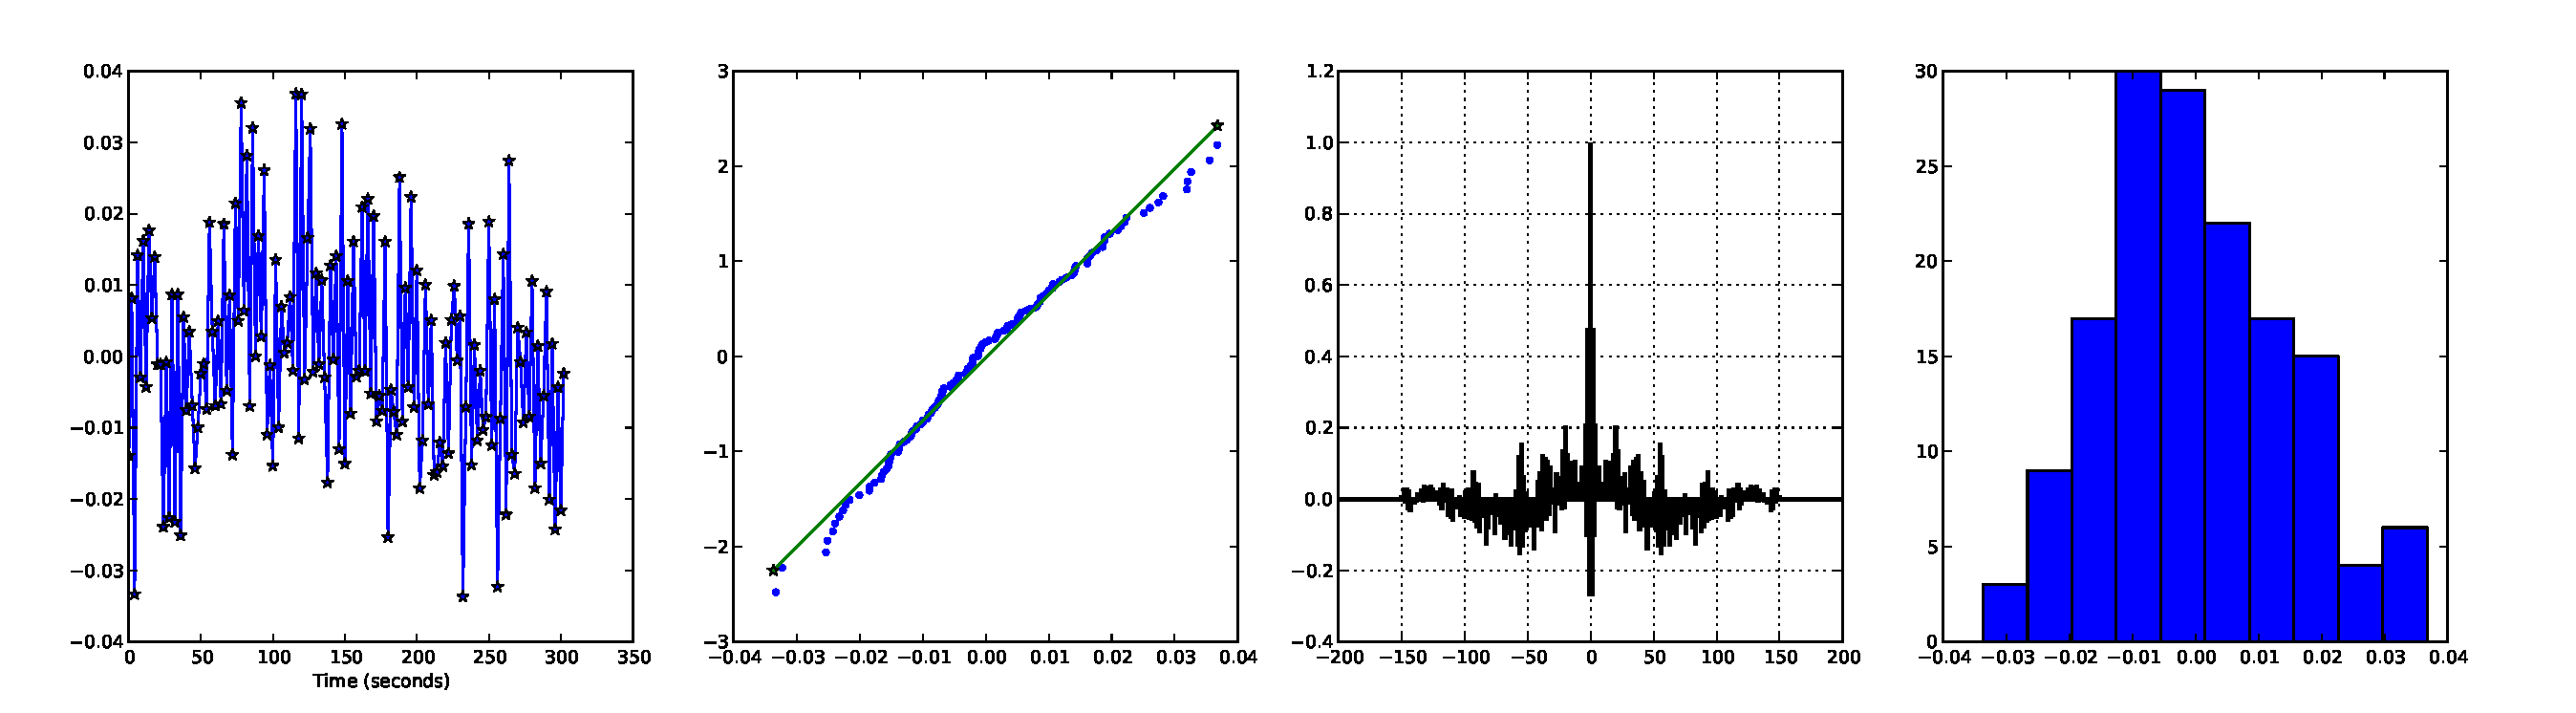
\includegraphics[trim=6cm 1cm 0 0cm,width=17cm]{images/noise_0009_19-24-10.pdf}}
%\subfigure{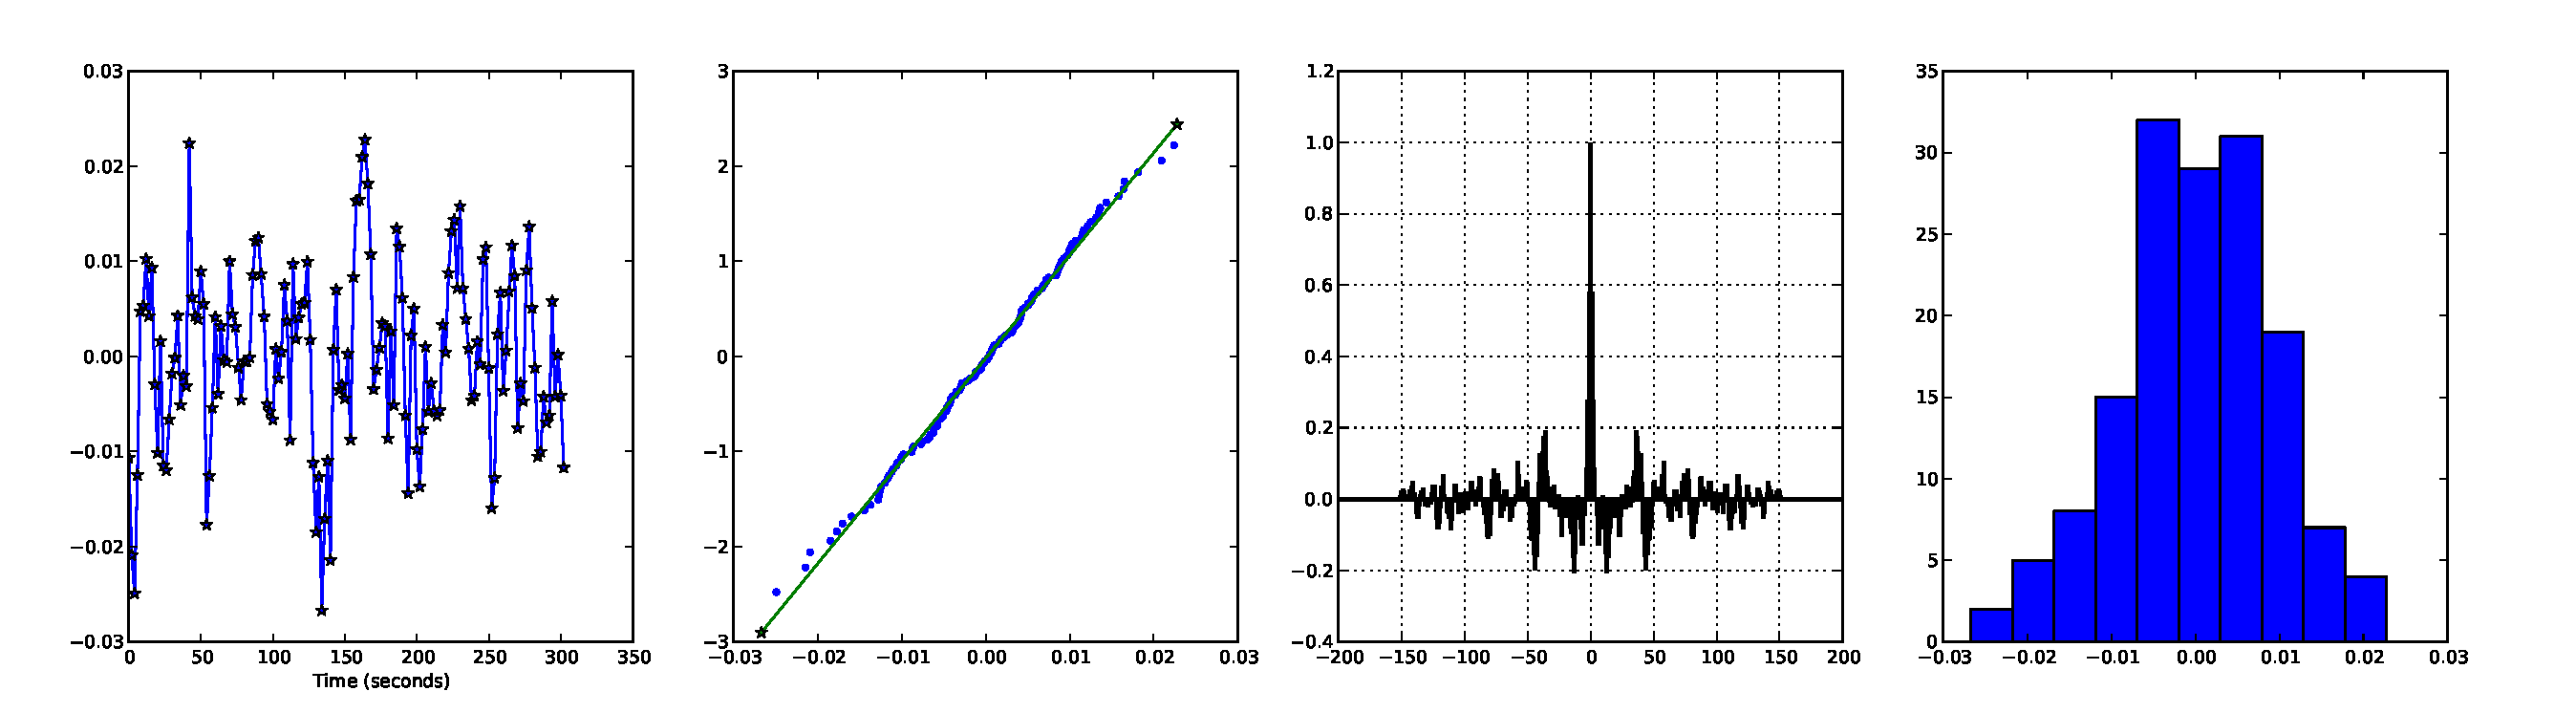
\includegraphics[trim=6cm 1cm 0 0cm,width=17cm]{images/noise_0009_20-45-18.pdf}}
%\subfigure{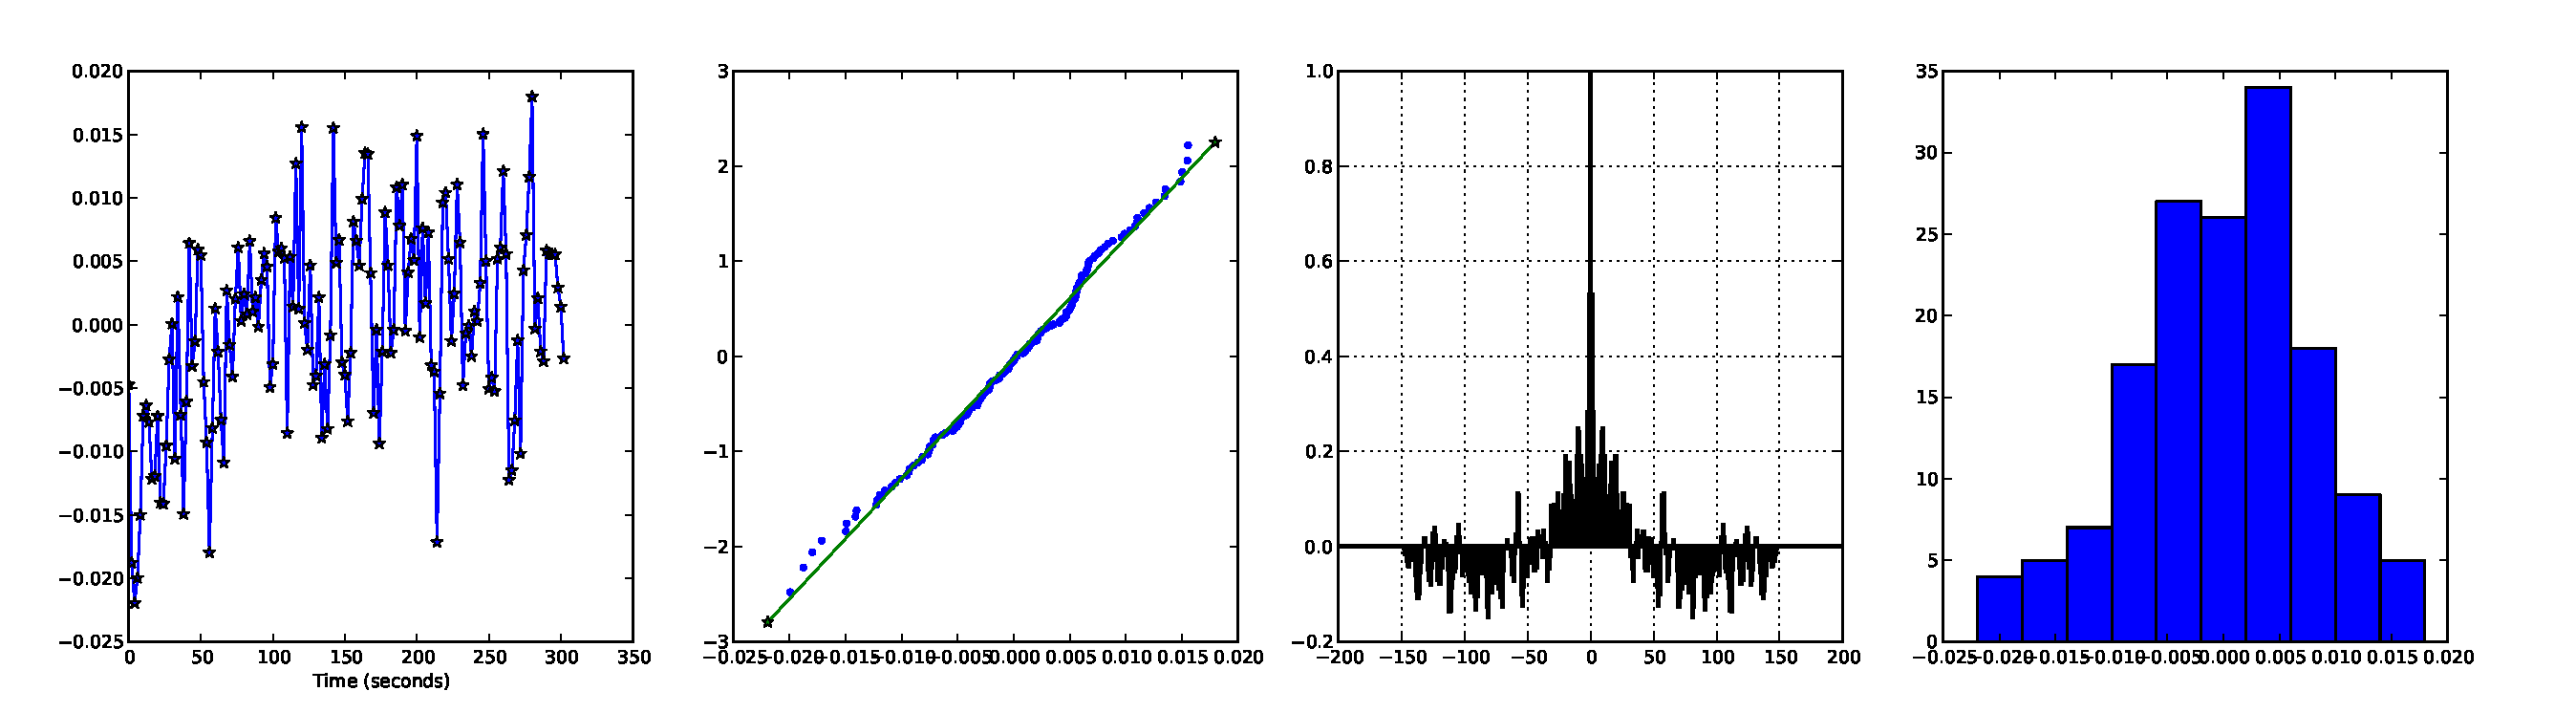
\includegraphics[trim=6cm 1cm 0 0cm,width=17cm]{images/noise_0009_23-47-18.pdf}}
%\subfigure{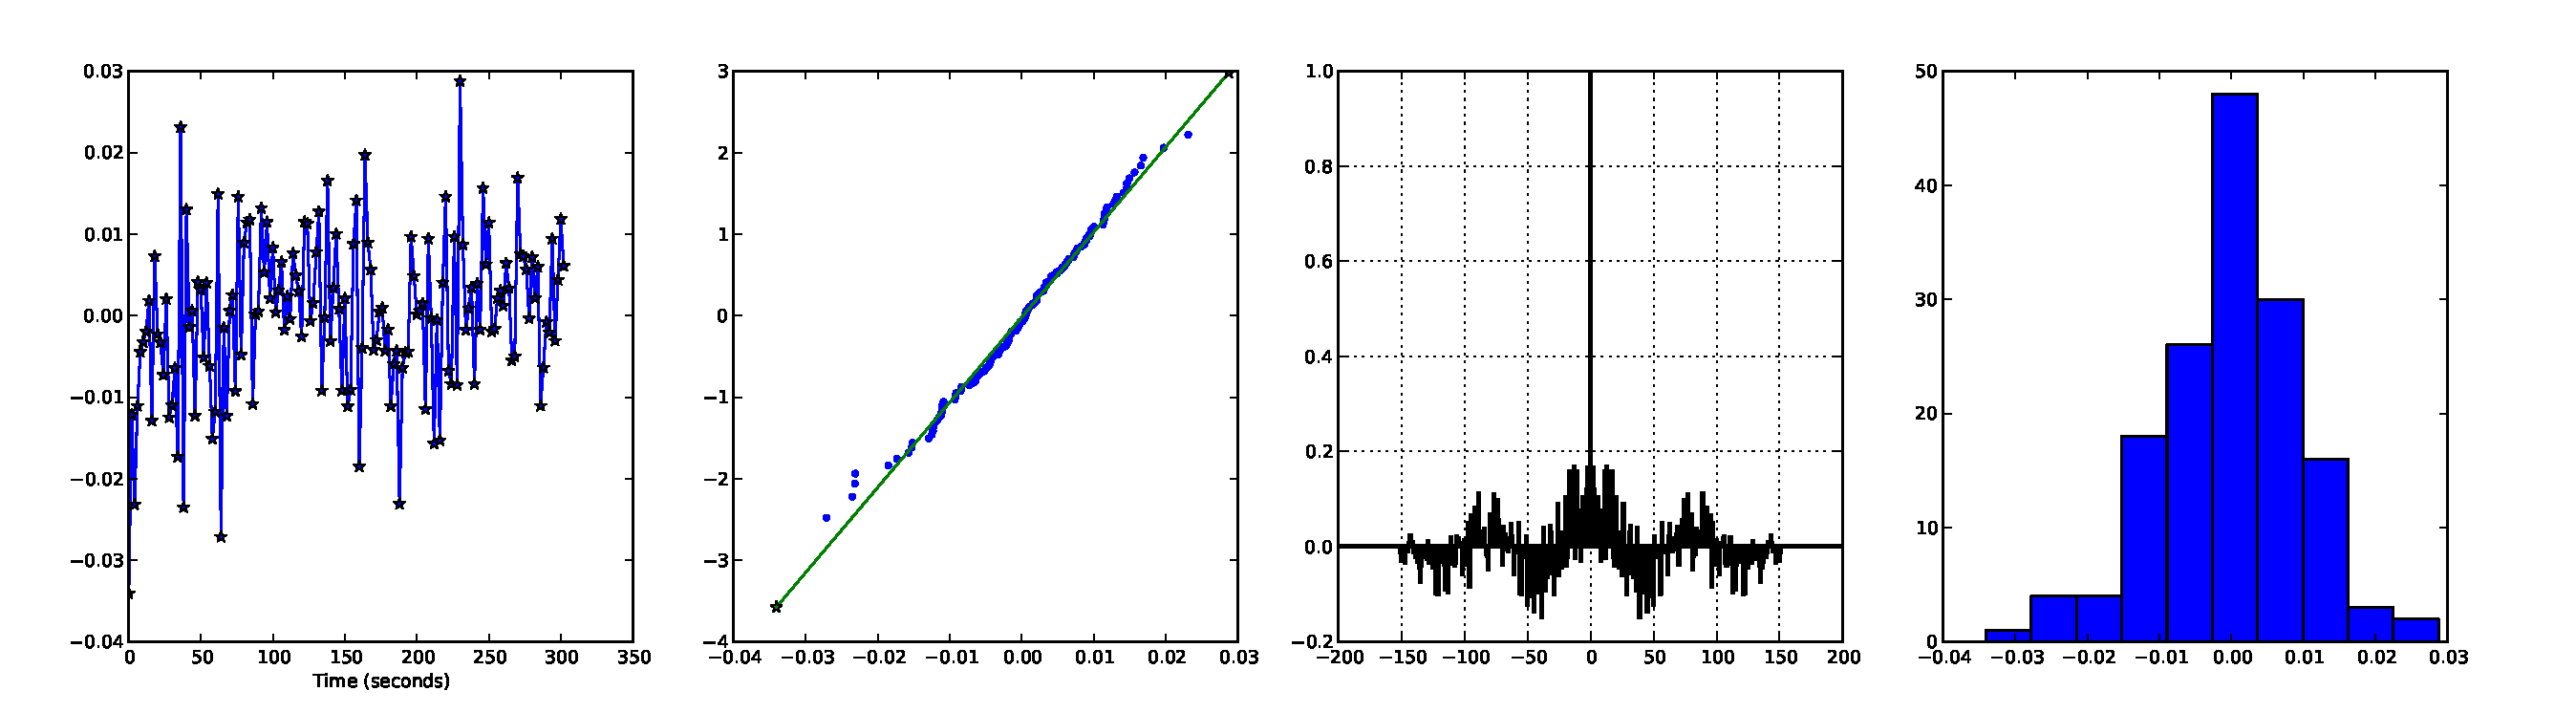
\includegraphics[trim=6cm 1cm 0 0cm,width=17cm]{images/noise_0009_35-49-9.pdf}}

\caption{Q-Q Plots of normalized resting state data}
\label{fig:QQDC}
\end{figure}

\begin{figure}
\centering
\subfigure[]{\label{fig:QQDDelta:A}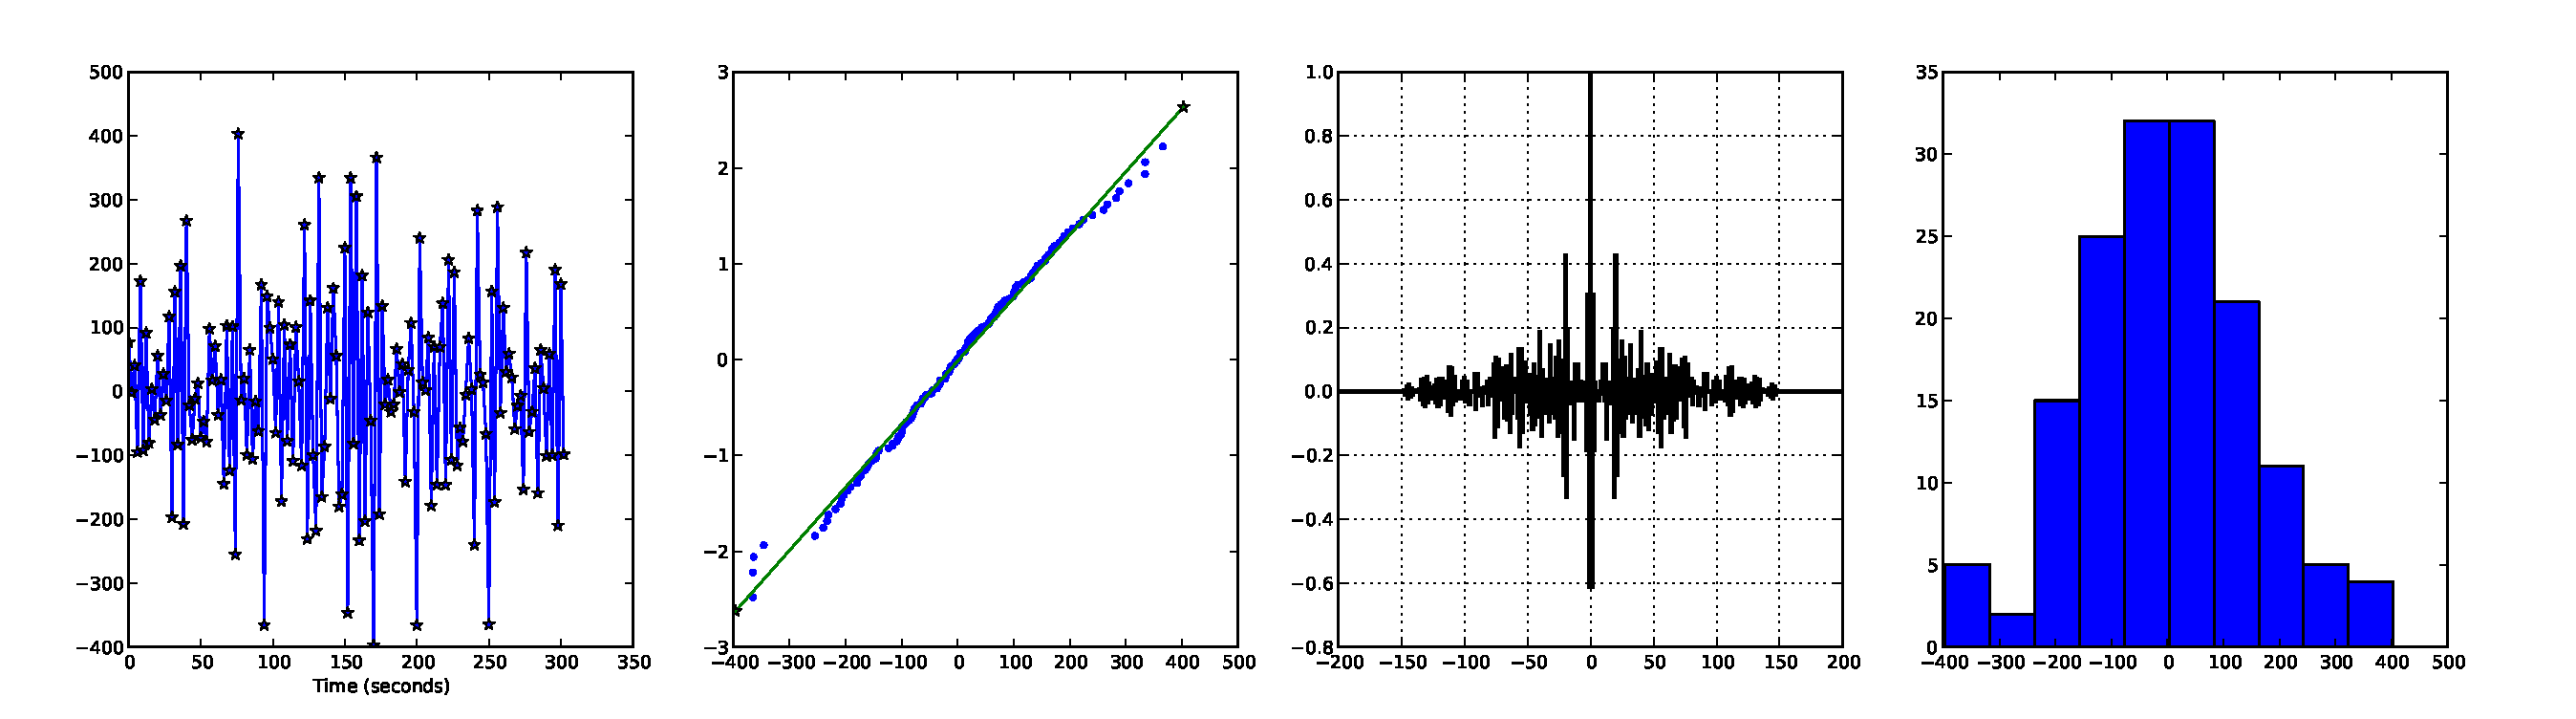
\includegraphics[trim=6cm 1cm 6cm 1cm,width=13cm]{images/noise2_0009d_29_49_9}}
\subfigure[]{\label{fig:QQDDelta:B}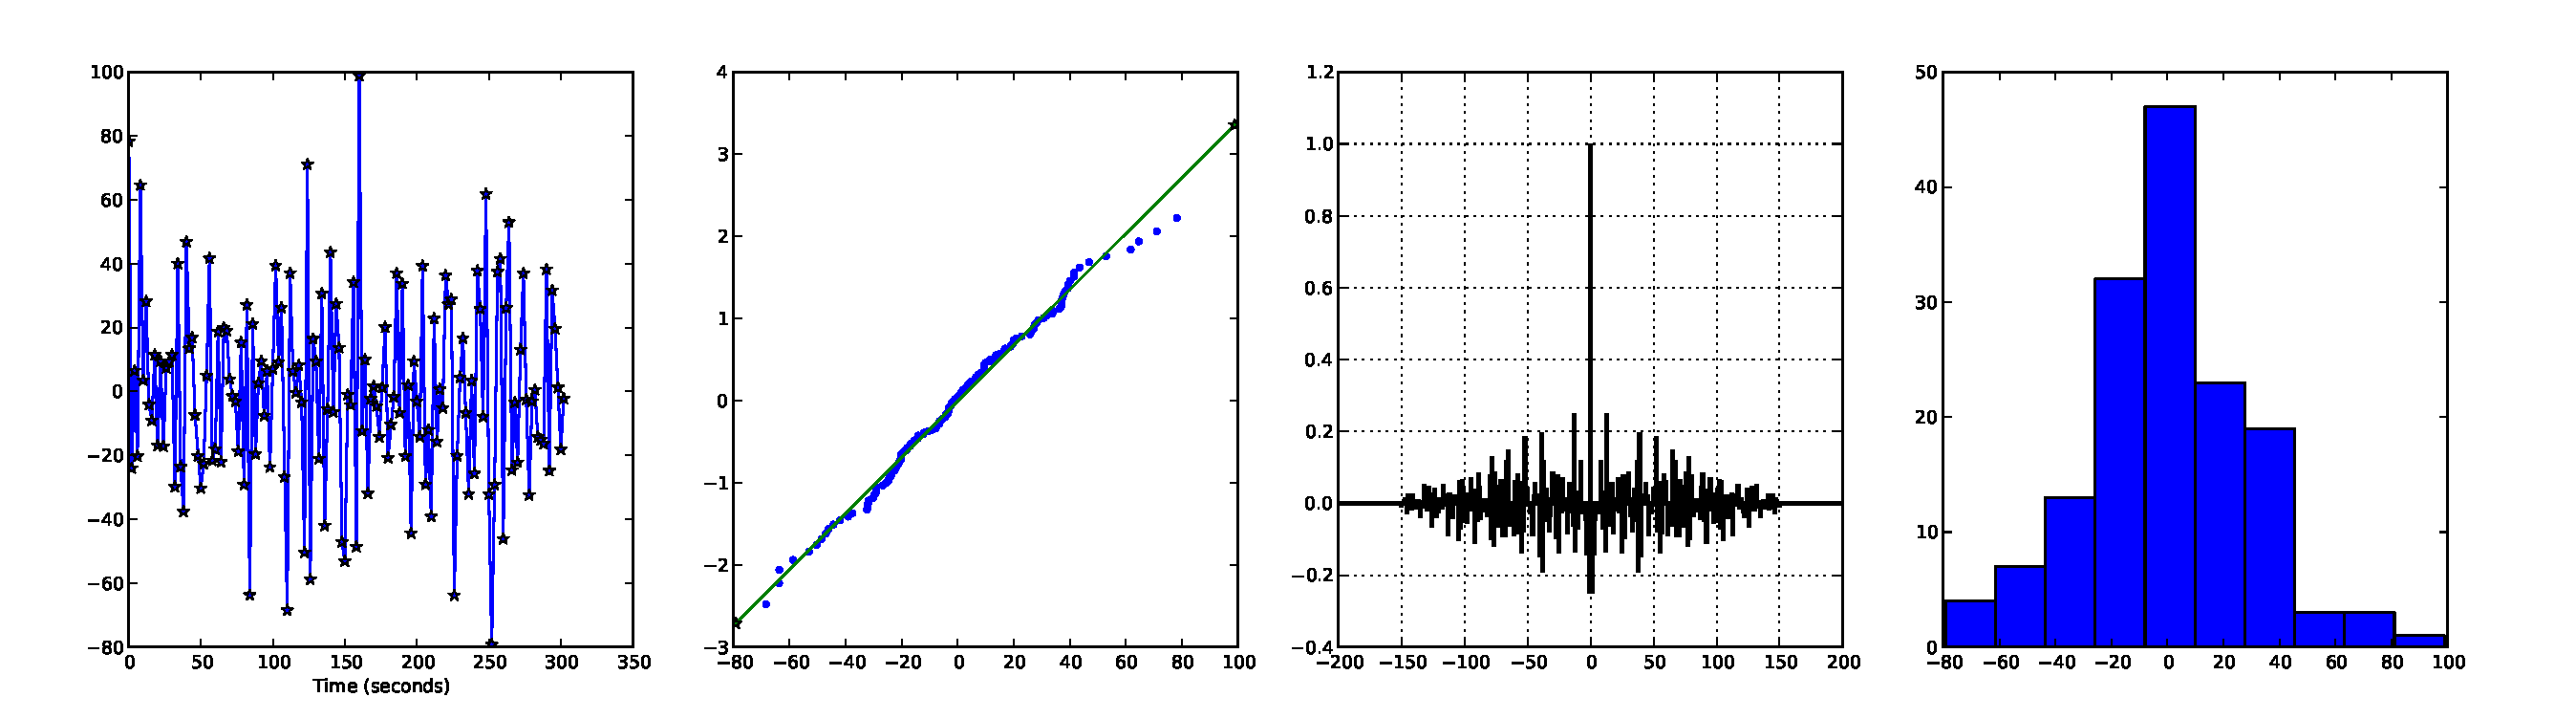
\includegraphics[trim=6cm 1cm 6cm 1cm,width=13cm]{images/noise2_0009d_34_43_24}}
\subfigure[]{\label{fig:QQDDelta:C}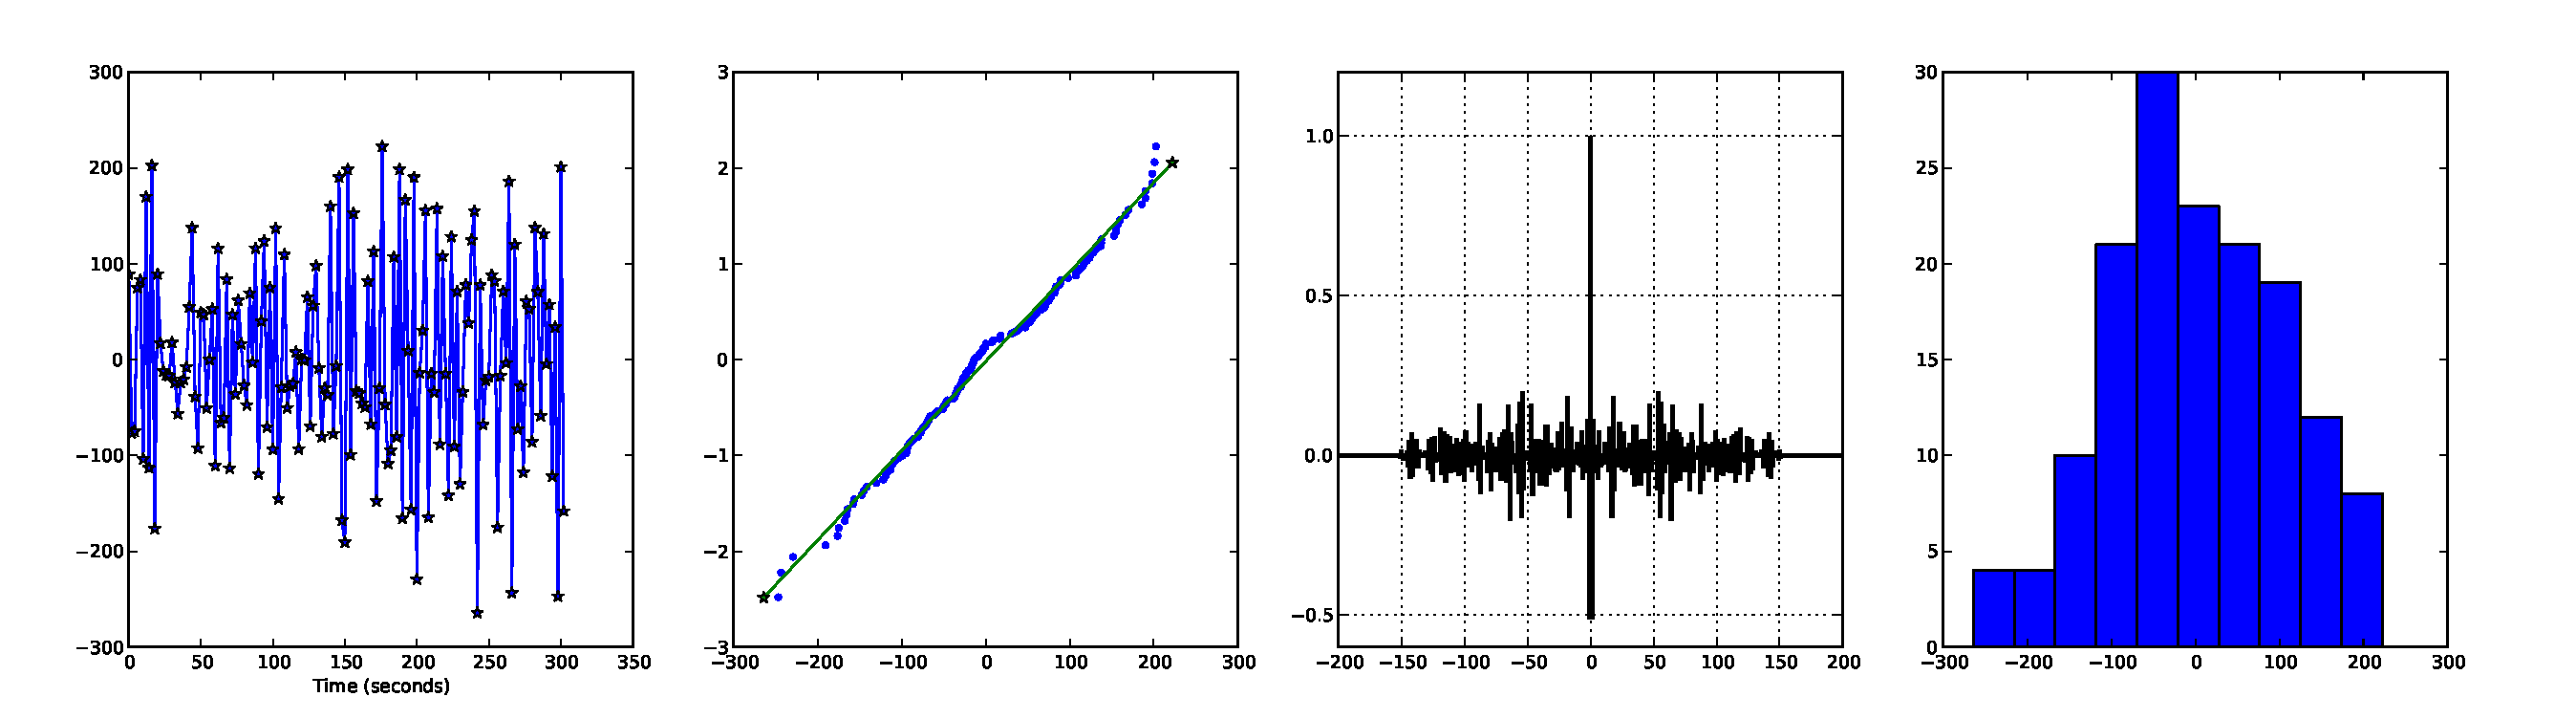
\includegraphics[trim=6cm 1cm 6cm 1cm,width=13cm]{images/noise2_0009d_22_38_23}}
\subfigure[]{\label{fig:QQDDelta:D}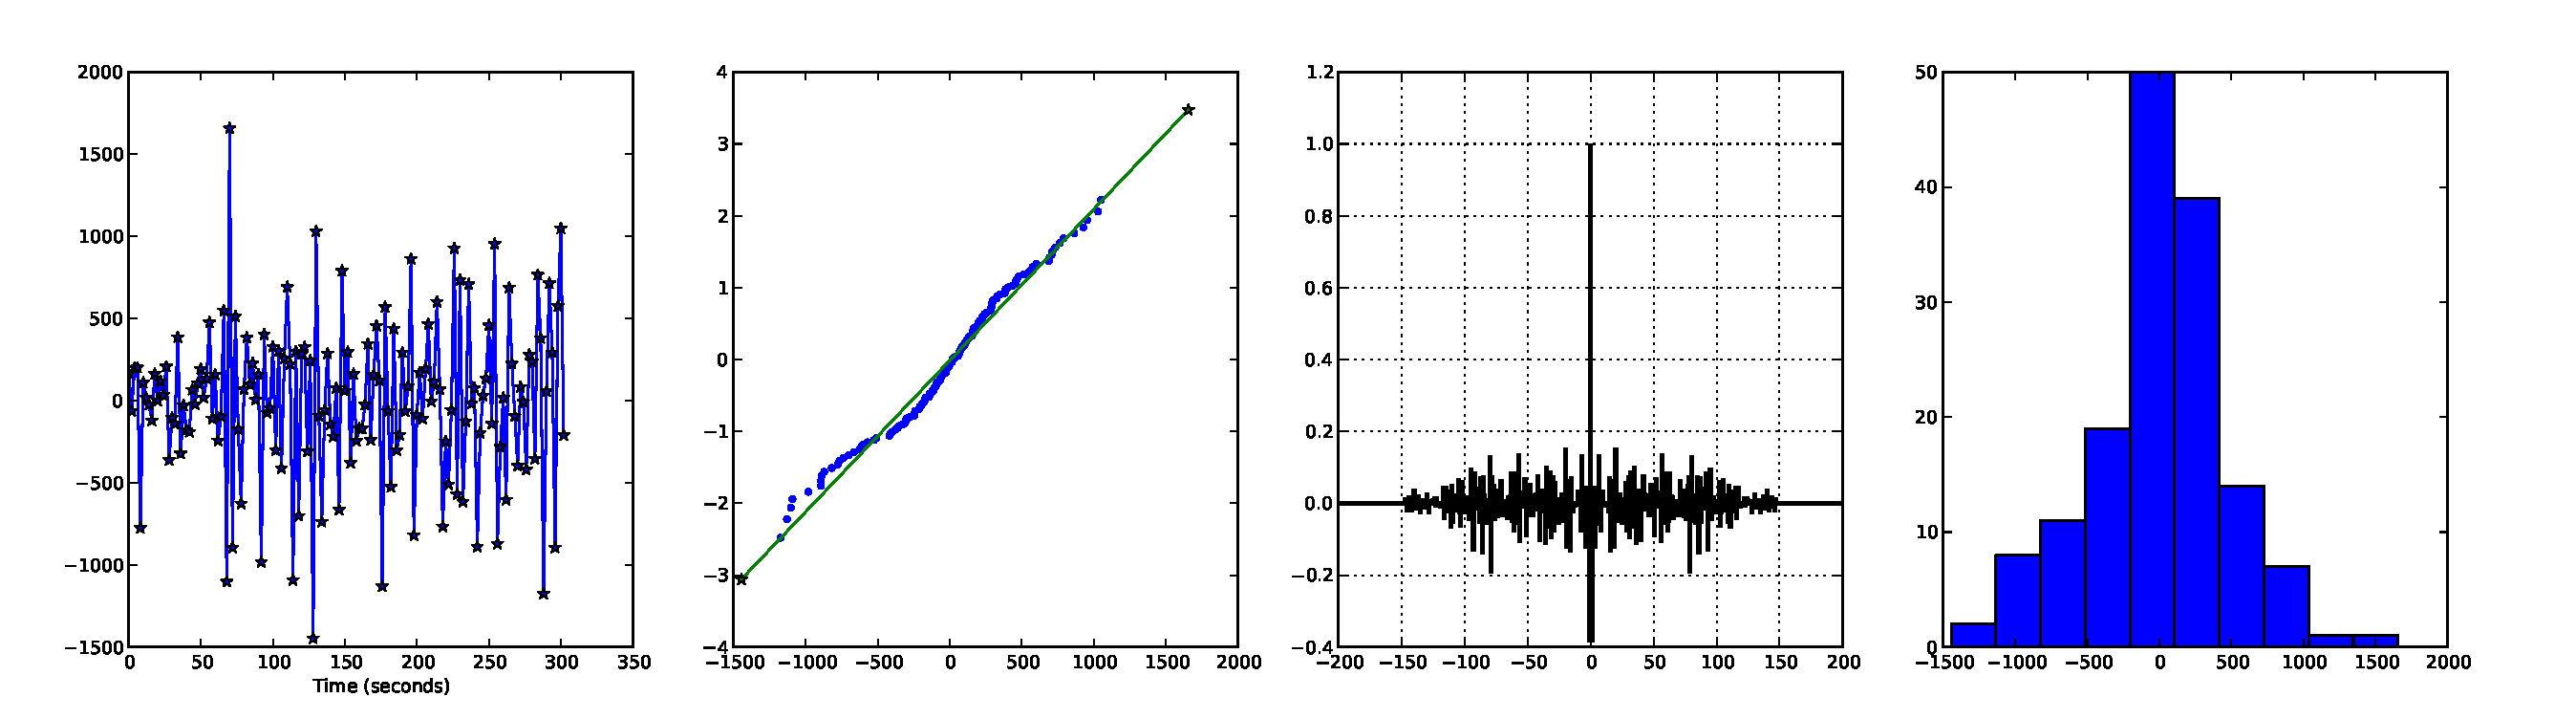
\includegraphics[trim=6cm 1cm 6cm 1cm,width=13cm]{images/noise2_0009d_37_29_24}}
\caption{Q-Q Plots of resting state data, using the BOLD signal steps.}
\label{fig:QQDelta}
\end{figure}


\begin{figure}
\centering
\subfigure[]{\label{fig:QQs:A}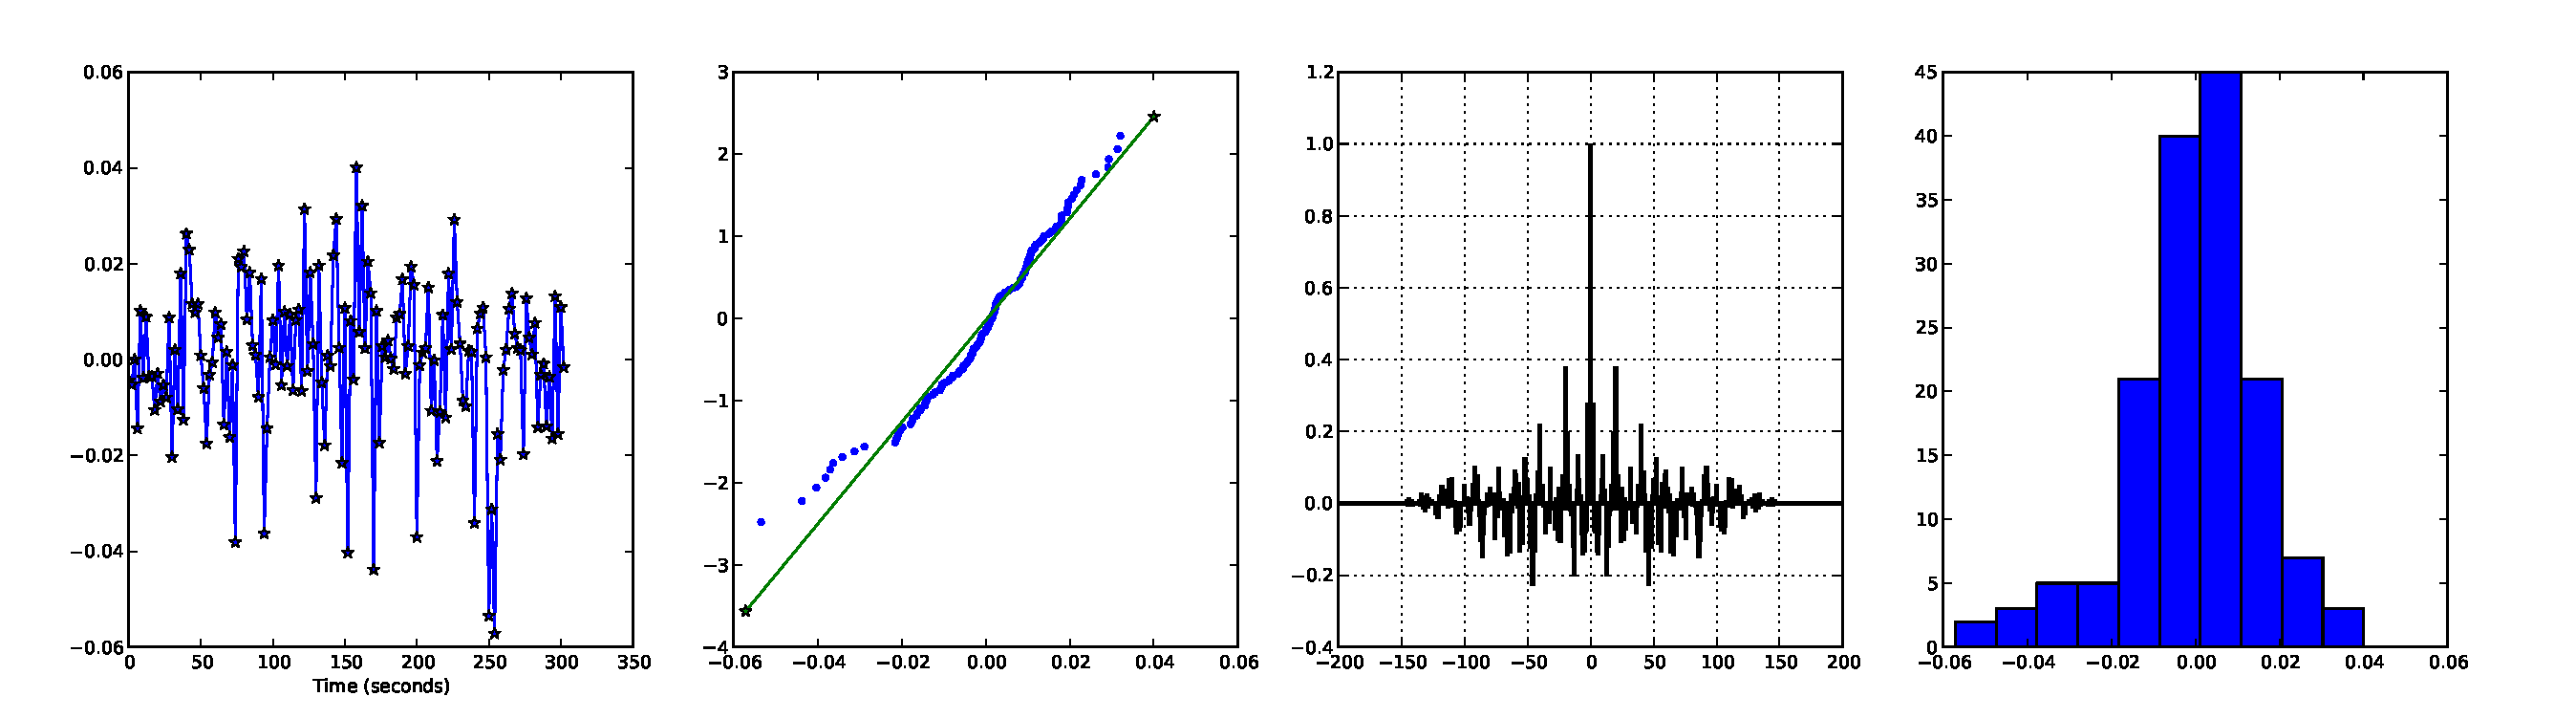
\includegraphics[trim=6cm 1cm 6cm 1cm,width=13cm]{images/noise2_0009s_29_49_9}}
\subfigure[]{\label{fig:QQs:B}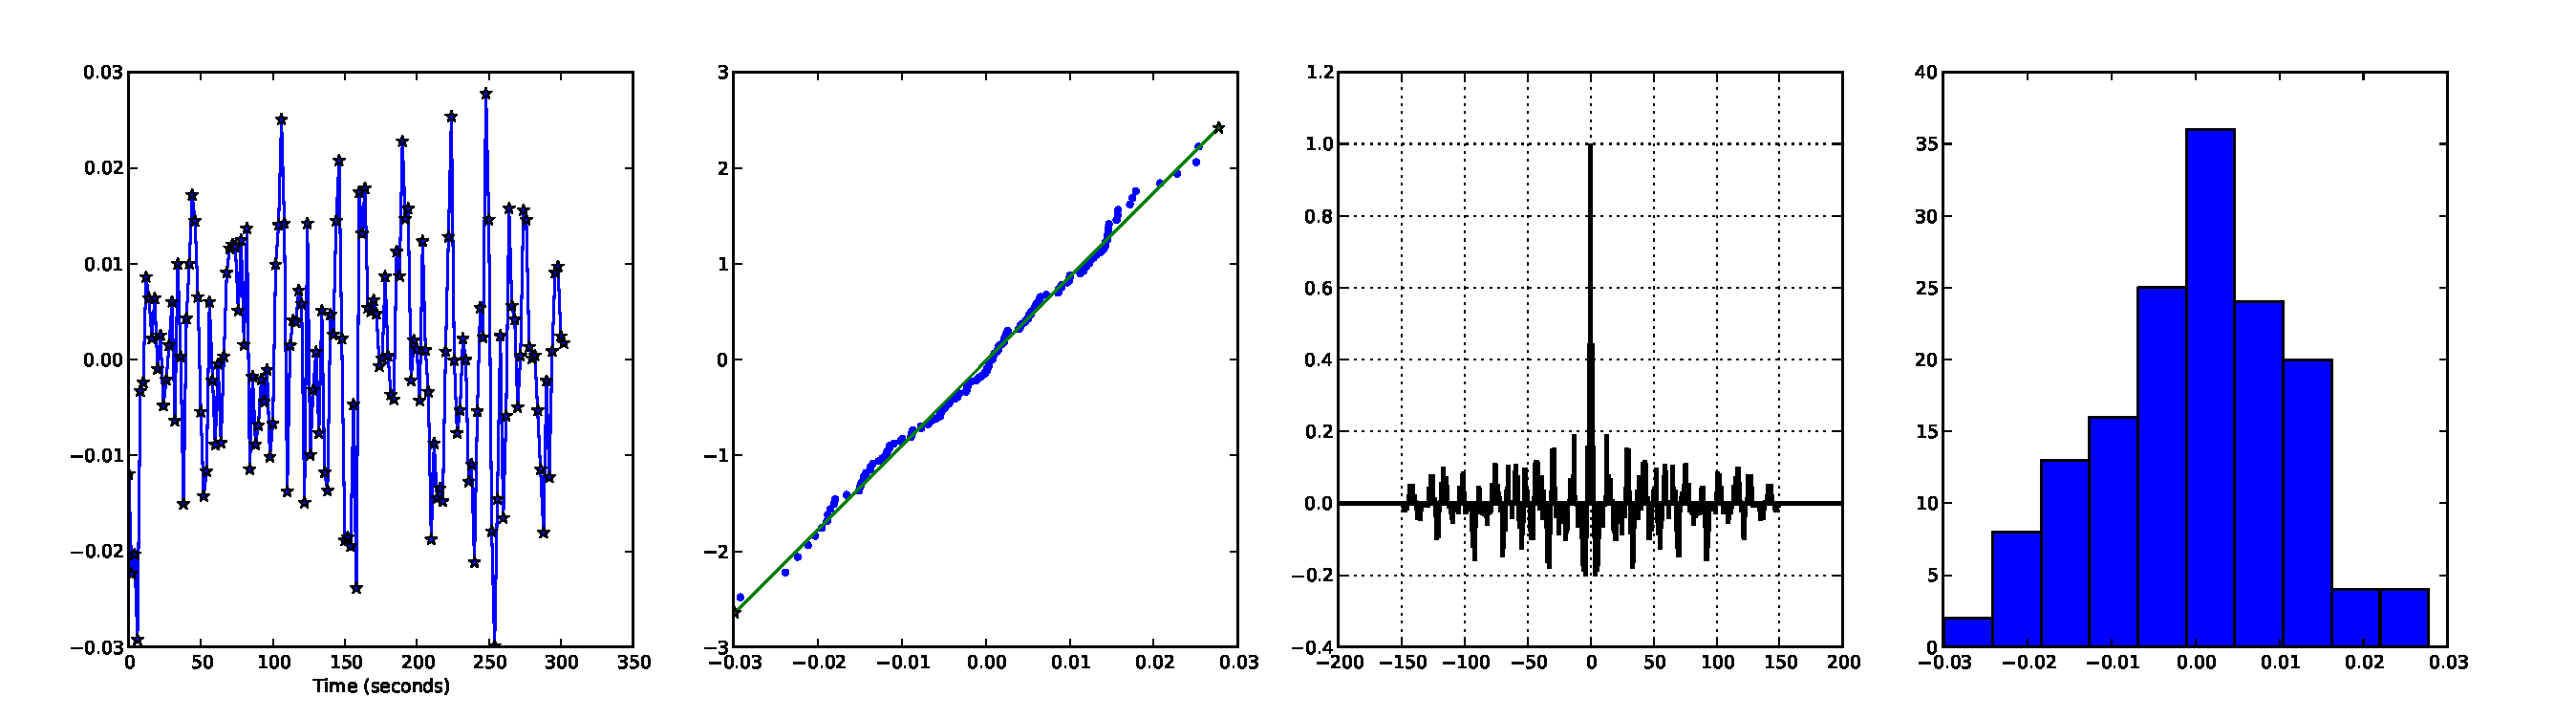
\includegraphics[trim=6cm 1cm 6cm 1cm,width=13cm]{images/noise2_0009s_34_43_24}}
\subfigure[]{\label{fig:QQs:C}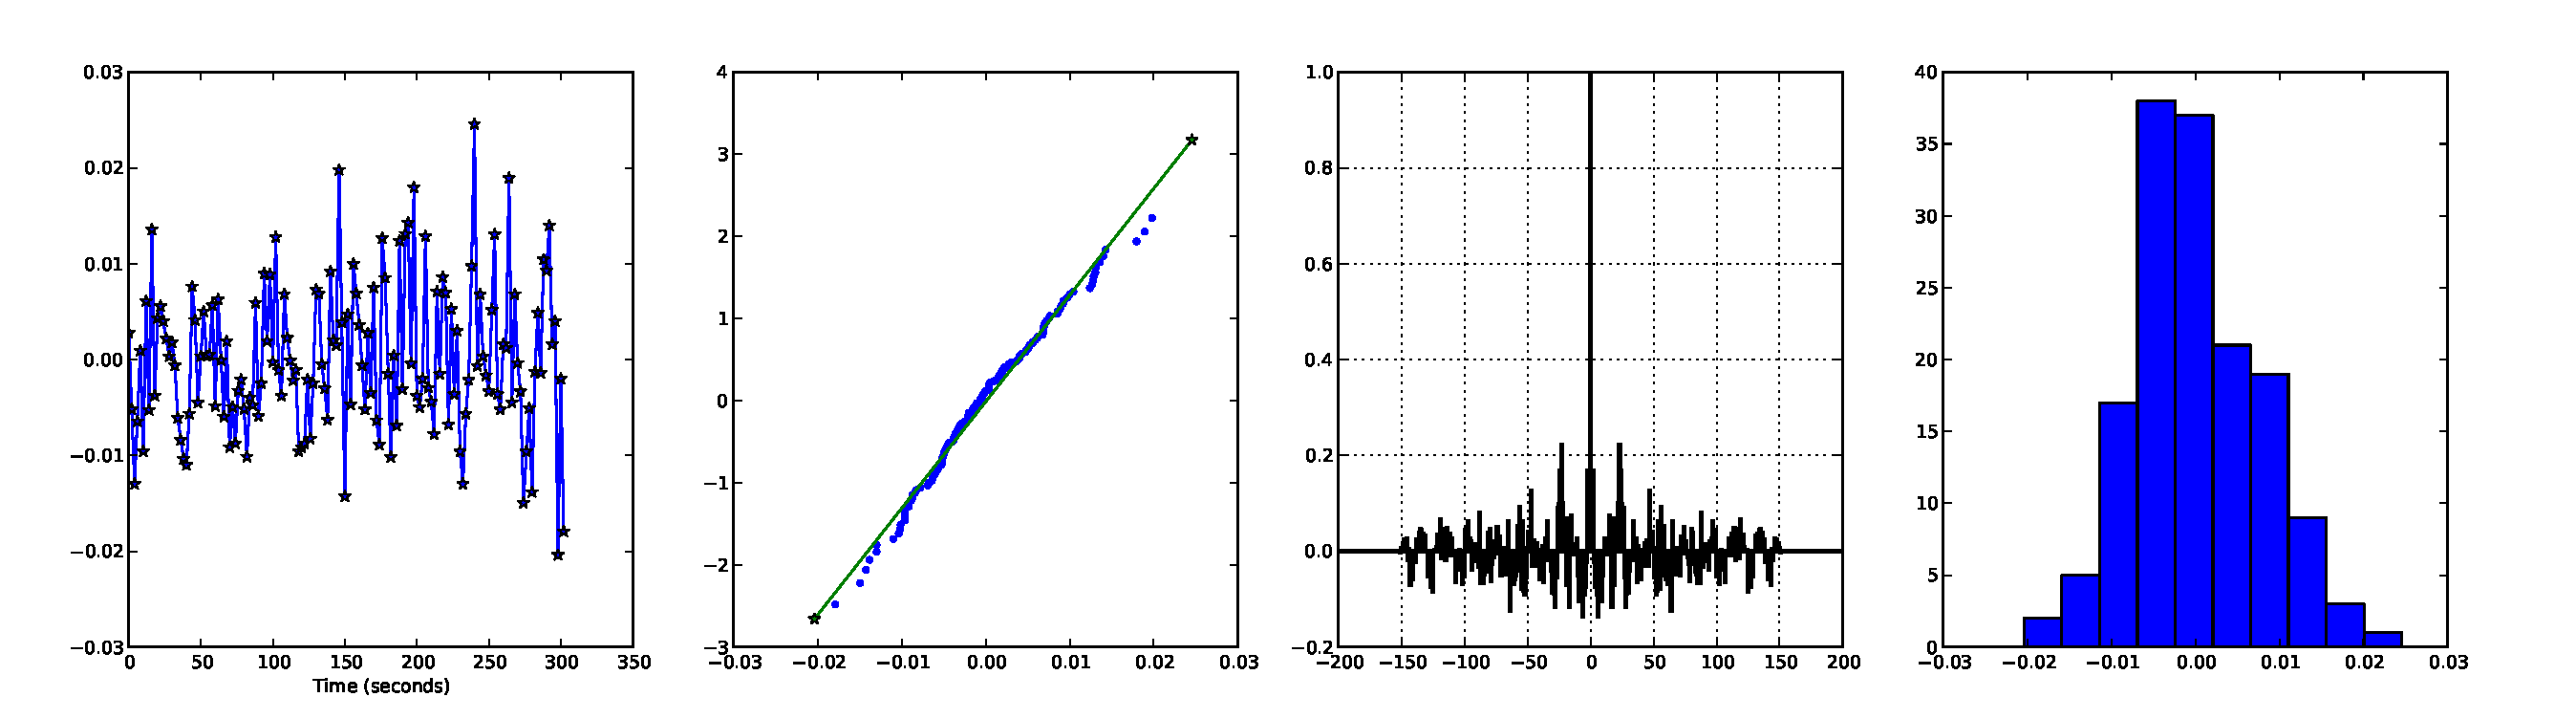
\includegraphics[trim=6cm 1cm 6cm 1cm,width=13cm]{images/noise2_0009s_22_38_23}}
\subfigure[]{\label{fig:QQs:D}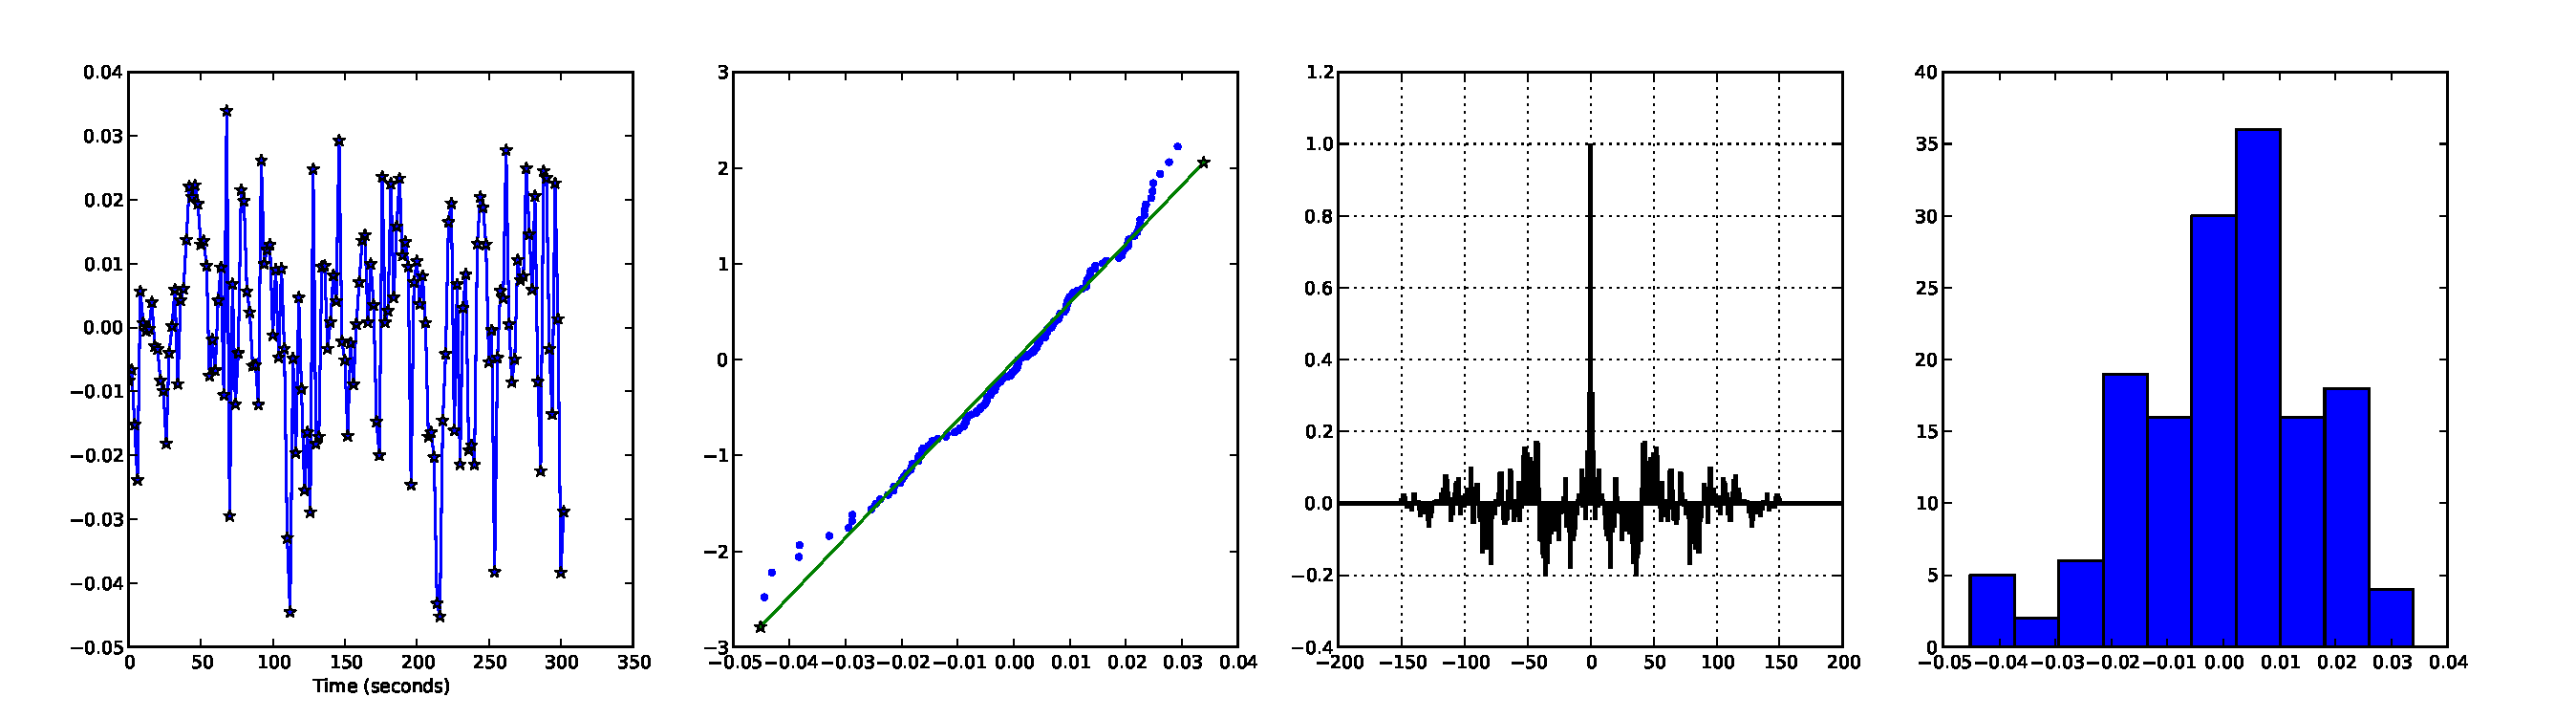
\includegraphics[trim=6cm 1cm 6cm 1cm,width=13cm]{images/noise2_0009s_37_29_24}}
\caption{Q-Q Plots of resting state data, after the de-trending}
\label{fig:QQSpline}
\end{figure}

Because most methods (including the one used in this paper)
assume the noise realizations are independent of each other, the autocorrelation 
is of particular interest (which is a necessary but not
sufficient condition for independence). Gaussianity is also a common
assumption made in studies of FMRI data, though that assumption is not
needed in this work. Regardless, comparing the distribution to a Gaussian
is informative, so Q-Q plots are used to compare example data with the
Normal distribution. Additionally, in FMRI data the noise is often considered 
to be Wiener \cite{Riera2003}. Recall that a Wiener random process is
characterized by steps that are Gaussian and independent. The simulations discussed in 
\autoref{sec:Single Voxel Simulation} make use of this, 
by adding a Wiener random process to the overall signal. To determine
whether the noise is in fact Wiener, the distribution of 
the steps were also plotted against a Gaussian. 

Finally, removal of the drift is often performed with a high pass filter,
so I also analyzed the distribution after subtracting a spline, (see \autoref{sec:Methods Preprocessing}).

\autoref{fig:QQDC} shows the 
results with a regression line fit to the points.
Recall that in a Quartile-Quartile (Q-Q) plot, if the points plotted on the 
x and y axes come from the same type of distribution, then all the points will
be collinear. Differences in the variance will cause the line to have a slope
other than 1, while differences in the expected value will cause the fitted line
to be shifted. In these Q-Q plots, the points are being compared to the standard
Gaussian distribution. Note that the points have all been 
normalized (changed to percent difference).

\autoref{fig:QQDC:A} and \autoref{fig:QQDC:B}
are well described by a Gaussian process with a small autocorrelation, but 
\autoref{fig:QQDC:C} and \autoref{fig:QQDC:D} are not. In particular the tails of \autoref{fig:QQDC:C}
do not seem to fit the Gaussian well. Also note the significant autocorrelation in
\autoref{fig:QQDC:C} and \autoref{fig:QQDC:D}. As expected, the noise is not strictly
Gaussian white noise.  On the other hand, the steps do conform rather
closely to the normal distribution.
As expected, most of the autocorrelation disappears for the step data. Given
that the steps seem to fit the Normal distribution, the low autocorrelation
indicates that the steps could be Independently Distributed. 
Therefore, the noise is consistent with a Wiener process. 

De-trending the time-series by subtracting a spline fit to the distribution
removed much of the autocorrelation present in \autoref{fig:QQDC:C} and \autoref{fig:QQDC:D},
though not perfectly. Though the distributions still do not exactly fit
the Normal, \autoref{fig:QQs:D} is much improved compared to \autoref{fig:QQDC:D}.
In all, the de-trending is effectively removing Wiener noise. 

\subsection{Detrending}
\label{sec:Detrend}
The non-stationary
aspect of a Weiner process, presumably the result of integrating some
$\nu_x$ is difficult to compensate for, and so many methods
have been developed to compensate for it. Tanabe et al. and Smith et al. 
demonstrated that this component is prevalent, and may in fact be an inherent  characteristic
of FMRI \cite{Tanabe2002, Smith1999}. It has been reported that in some studies as 
many as half the voxels 
benefited from detrending \cite{Smith2007}. In a head to head comparison, 
Tanabe et al.  showed that in most cases subtracting off
a spline worked the best \cite{Tanabe2002}. 
The benefit of the spline versus wavelets, high pass 
filtering or other DC removal techniques is that the frequency response is not set.
Rather, the spline is adaptive to the input. Unfortunately no method will 
perfectly remove noise, and no method will leave the signal untouched.

The method I used to calculate the spline was picking one knot for every 20
measurements in an image. Thus a 10 minute session at a repetition time of 
2.1 seconds would have 19 knots. The first and last knots were each 
given half the number of samples as the rest of the knots; which were all 
located at the center of their sample group. The median of each sample group
was then taken and used as the magnitude for the group. Taking the median 
versus the mean seemed to work better, given the presence of outliers. 
There is potential to optimize the spline further using a canonical 
HRF to find resting points; however, the experiment would have
to be designed with this in mind. 

Problematically, after removing the DC component of the signal,
by definition the signal will have a median near zero. 
Unfortunately this is not the natural state of the BOLD signal. More specifically,
when the signal is inactive, the BOLD response should be at 0\% change from
the base level; activation may then increase, or for short periods decrease from this base.
Because most of the BOLD signal is above baseline, after removing the spline
the resting state will be below 0\%.  
One method of accounting for this is to simply add a DC gain model parameter.
Like all the other model parameters, with enough measurements, the particle filter
would be able to settle on a good estimate. Yet adding another dimension increases the
complexity of the model, when the parameter is relatively easy to estimate
by visual inspection.  In this work a simpler approach was used. To determine
the DC gain I used a robust estimator of scale. The Median Absolute Deviation (MAD)
proved to be accurate in determining how much to shift the signal up
by. I tested both methods during the course of analysis, and found that the increase 
in model complexity far outweighed the slight increase in flexibility. Other
methods may work better, however the MAD worked well, 
as \autoref{fig:PreprocessedLowNoise} and \autoref{fig:PreprocessedHighNoise} show. 

\begin{equation}
y_{\text{gain}, 0:K} = 1.4826\underset{i=0:K}{\text{median}}(y_i - \text{median}(y_{0:K}))
\label{eq:mad}
\end{equation}

A serious concern when adding constant values to 
real data is whether this will create false positives. This is a legitimate
concern; however, a boosted response does not effect how well the BOLD model 
predicts the actual measurements; and as mentioned before, the DC signal of FMRI
is never used. 

%\subsection{Linearizing Noise}
%\label{sec:Methods Delta Based Inference}
%The alternative to these sorts of low frequency manipulation is to
%go around the problem in another way. Here, I propose a 
%different method of dealing with the drift. 
%Instead of comparing the direct output of the particle filter with the direct
%measurement, the algorithm would compare the change in signal over a single TR,
%with the result of integrating the model for the same period. 
%In most signal processing cases this would be foolish, but that is because the 
%general assumption is that all noise is high frequency. Considering 
%the fact that every BOLD analysis pipeline uses a high pass filter,
%whereas low poss temporal filter are rarely applied, it makes sense
%that a derivative type method could work. The benefit of particle filters
%is that they are a robust method of inference, and I would assert 
%that the particle filter ought to be given as \emph{raw} data as possible. 
%While taking direct measurements
%without de-trending would give awful results, using the difference removes the 
%DC component and turns what is usually assumed to be a Weiner process into 
%a simple Gaussian random variable. 
%
%\begin{equation}
%\Delta y = y(t) - y(t-1) = g(x(t)) - g(x(t-1)) + \nu_y(t) - \nu_y(t-1) + \nu_d(t) - \nu(t-1)
%\label{eq:measass_delta}
%\end{equation}
%
%Even if $\nu_d$ is some other additive process, the difference will still be closer
%to I.I.D. than a Wiener process, as the autocorrelation of the $\delta y$ shows
%in \autoref{fig:QQDelta} in \autoref{sec:Introduction Noise}. 
% All the assumptions made originally
%for the particle filter still hold, and all of the parameters may be distinguished based on
%the step sizes, thus it is not unreasonable to consider matching the string of step sizes
%rather than string of direct readings. 
%
%\begin{figure}
%\label{fig:FrequencyGraphs}
%\caption{frequency response graphs, highlighting noise frequency range and signal frequency range}
%\end{figure}

\section{Particle Filter Settings}
There are quite a few options when using a particle filter; therefore this
section will discuss the design choices made in this work.

\subsection{Prior Distribution}
\label{sec:PriorDist}
For the BOLD model described in \autoref{sec:BOLD Physiology}, several
different studies have endeavored to calculate parameters. The results
of these studies may be found in \autoref{tab:Params}, and the methods 
used for each may be found in \autoref{sec:Prior Works}. Unfortunately,
Friston et al. only studied regions deemed active by the General 
Linear Model; and most other research (including \cite{Friston2001}) used these results as 
the source for their priors \cite{Friston2000}. 
The one exception is to this is Johnston et al. which came to a extremely different
distributions \cite{Johnston2008}. For a particle filter, the choice of a prior is
the single most important design decision. A very wide prior will require
more particles to be sufficiently dense, a very thin (low variance) prior may miss
the true parameters. Consequently, for this work it was natural
to use priors that would give results consistent with previous works
\cite{Friston2000}. This constrains the usefulness of the model to
areas that fall within the prior distribution, yet allowed results
to be comparable to other works. There is a significant need for better
estimates of the physiological parameters; and, while physical experiments
may not be possible, it would not be unreasonable to do a study with
exhaustive simulated annealing or hill climbing tests for multiple
regions and multiple patients. That said, a significant amount of
indeterminability exists in the parameters, which is discussed in 
\autoref{sec:Single Voxel Simulation}

\begin{figure}
\centering
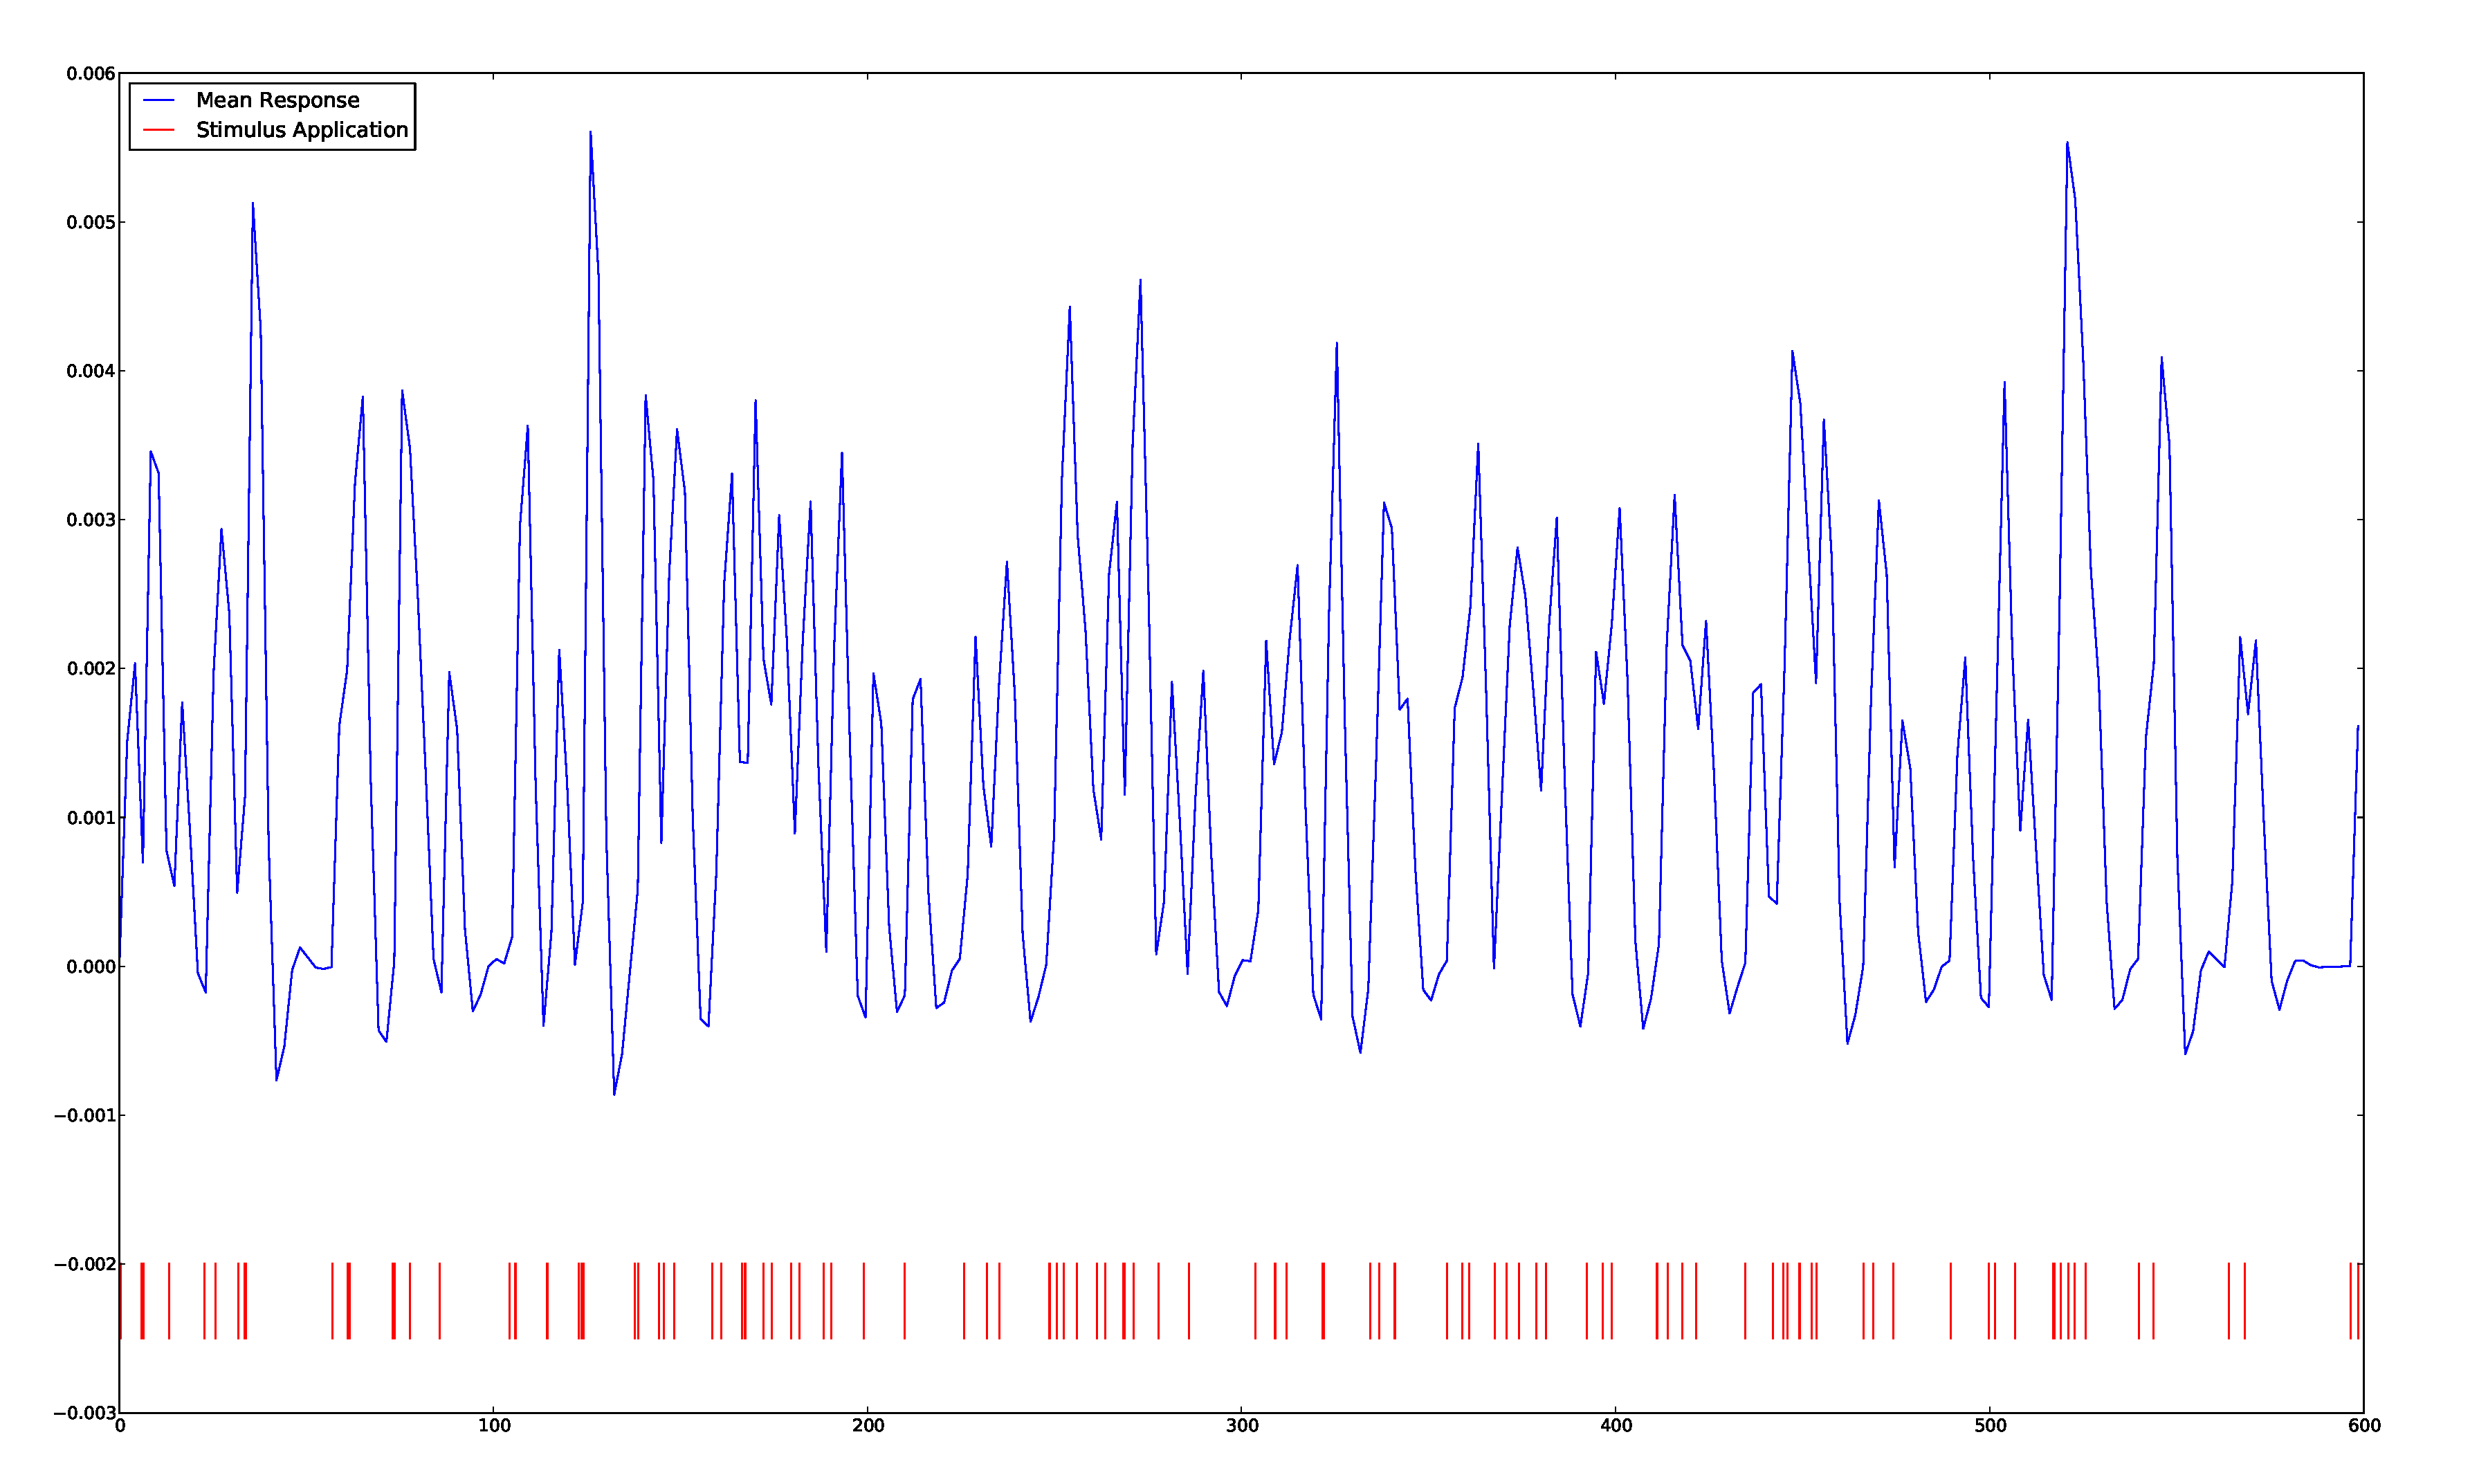
\includegraphics[trim=6cm 2cm 6cm 2cm,width=15cm]{images/mean_response}
\caption{Response to $0.1s$ impulses with the mean parameters from \cite{Friston2000}}
\label{fig:MeanResponseF}
\end{figure}

\begin{figure}
\centering
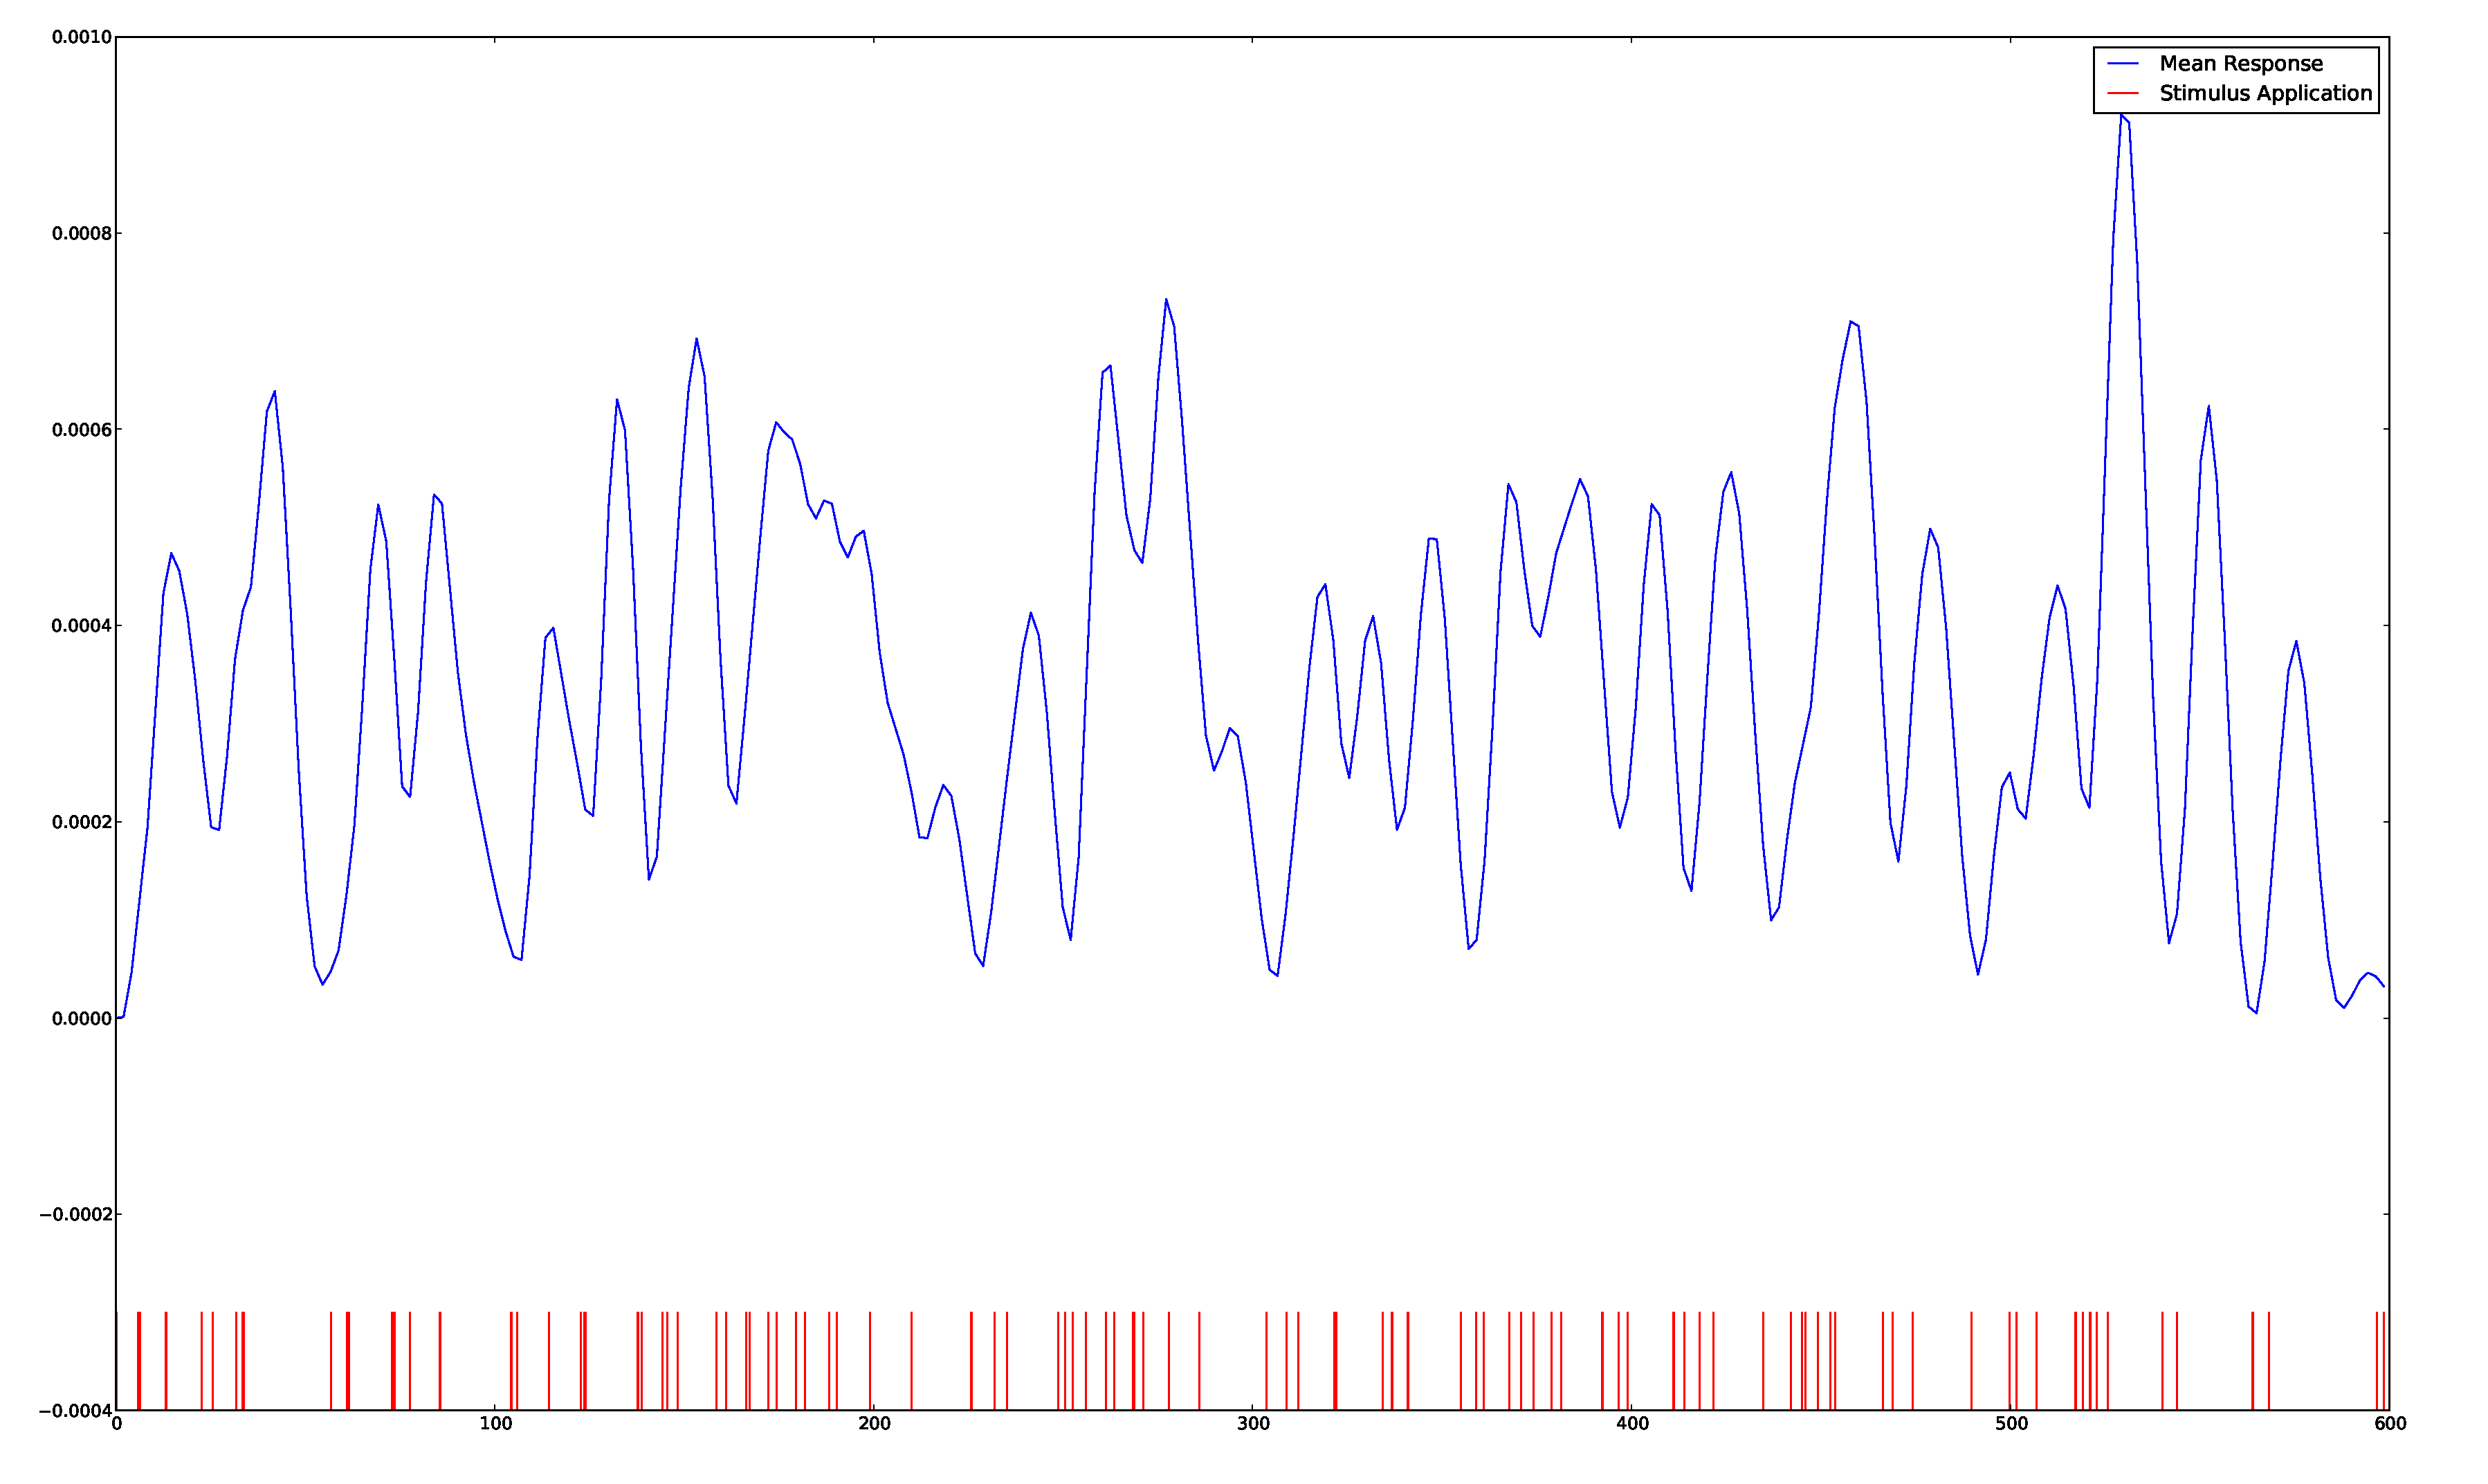
\includegraphics[trim=6cm 2cm 6cm 2cm,width=15cm]{images/mean_response_johnston}
\caption{Response to $0.1s$ impulses with the mean parameters from \cite{Johnston2008}}
\label{fig:MeanResponseJ}
\end{figure}

The differences between the parameter estimates of Johnston et al. and 
Friston et al. are clearly visible in \autoref{fig:MeanResponseJ} and 
\autoref{fig:MeanResponseF} \cite{Johnston2008,Friston2002}. 
Therefore, to account for these discrepancies, I used tests on
real data to adjust the distributions from those arrived at in 
Friston et al. \cite{Friston2002}. In tests on real data, the Johnston et al.
distributions never converged to meaningful BOLD estimates.
The priors used in the particle filter may be found in \autoref{tab:Prior}.

\begin{table}[t]
\centering
\begin{tabular}{|c || c | c | c |}
\hline 
Parameter & Distribution & $\mu$ & $\sigma$ \\
\hline
$\tau_0$ & Gamma & .98 & .25 \\
$\alpha$ & Gamma & .33 & .045\\
$E_0$    & Gamma & .34 & .03  \\
$V_0$    & Gamma & .04 & .03 \\
$\tau_s$ & Gamma & 1.54  & .25\\
$\tau_f$ & Gamma & 2.46  & .25\\
$\epsilon$ & Gamma & .7  & .6 \\
\hline
\end{tabular}
\caption{Prior distributions used in the particle filter.}
\label{tab:Prior} 
\end{table}

Note that although the mean remains the same for all the 
parameters other than $\epsilon$, the standard deviation were
adjusted based on tests with real data. Also, the state variables
were all assumed to be at rest at the beginning of the simulation.

It is also import to use enough particles to obtain a 
sufficiently dense approximation of the prior. For 7 dimensions,
getting a dense prior is difficult. Insufficiently
dense particles will result in inconsistent results. Of course the
processing time will scale up directly with the number of particles.
A dense initial estimate is important so that some particles land
near the solution; but as the variance decreases the number of 
particles needed decreases as well. Thus, as a heuristic, initially
the number of particles was set to 16,000, but after resampling,
the number of particles was dropped to 1,000. Typically during the 
first few measurements the variance drops precipitously because
most particles are far from a solution.  The particles that are left are in a
much more compact location, allowing them to be estimated with 
significantly fewer particles. These numbers aren't set in stone,
and depending on the complexity of the system or desired accuracy
they could be changed; however, they seem to be the minimum that
will give consistent results.

\subsection{Resampling}
\label{sec:Resampling}
The algorithm for resampling is described in \autoref{sec:Particle Filter Resampling}.
When regularizing, the Gaussian kernel is convenient,
because it is simple to sample from and long tailed.
As discussed in \autoref{sec:Particle Filter Resampling},
as long as resampling is kept as a last resort, some over-smoothing
doesn't impair convergence. Therefore, for this work I chose a Gaussian kernel of
bandwidth equal to the original distribution's covariance. This 
applies a large amount of smoothing to the distribution; however, on average
resampling was only applied every 20 to 30 measurements, and because randomization
is being applied to model updates this gives the filter some mobility. 

Resampling is a not strictly necessary, but it increases the effectiveness
of the particle filter by adjusting the support to emphasize areas
of higher probability. Resampling is slow because it requires redrawing
all the particles. It also closes off avenues of investigation, and is
designed to over-smooth to prevent overly thinning the support. For all these
reasons, resampling was only performed when the $N_{eff}$ dropped below
50 (for 1000 particles).  As a measure against sharp drops in the $N_{eff}$ 
caused by a large spike in error, resampling was only performed when 
two consecutive low ($<50$) $N_{eff}$'s were found. 

\subsection{Particle Deprivation}
\label{sec:Particle Deprivation}
To prevent particle deprivation, which may happen even with a good
estimate of the prior distribution, a method of rescuing the particle
filter from this state was used. When particle deprivation was detected,
resampling was performed with a saved version of the covariance matrix (from
the previous time step). This allowed for the particles to be re-scattered
without having to go all the way back to the prior distribution. Particle 
deprivation was defined by $N_{eff}$ dropping to $1$.

\subsection{Choosing $P(y_k | x_k)$}
\label{sec:Methods Weighting Function}
The choice of $P(y_k | x_k)$ is the second most important design decision, behind 
the prior. While the conventional choice for an unknown distribution is the 
Gaussian, there are reasons why it may not be the best in this case.  
As noted in \autoref{sec:Introduction Noise}, the noise is not strictly Gaussian,
nor is it strictly Wiener. As with any unknown noise however, it is necessary 
to make some assumption. If the weighting function ($P(y_k | x_k)$) exactly
matches the measurement error, then the ideal particle filter will result.
Particles with $x_k$'s that repeatedly estimate $y_k$ with large residual 
will quickly have weights near 0. Thus, a weighting function that
exactly matches $P(Y(t) | X(t))$ will easily and correctly throw out invalid
particles.  The cost of choosing an overly broad distribution for this
function is slow convergence.  On the other hand, an overly thin 
distribution will lead to particle deprivation (all particles
being zero-weighted). Three weighting functions were 
tested. In addition to the Gaussian I also tested the Laplace and Cauchy
distributions, both of which have wide tales. 
Wider tailed distributions don't down-weight
particles as fast; and thus converge more slowly. 
The Laplace distribution also has the
benefit of a non-zero slope at the origin; meaning it 
differentiates between particles even near the origin.

After trial and error, for this work I chose the Gaussian with a standard deviation 
of $0.005$. Although using an adaptive weighting function
might be better, in tests this often led to unpredictable results. 
With some work it may be possible to set the standard deviation by
taking a small sample from resting data and using the sample standard deviation.
In this work, however, I set the standard deviation manually at $0.005$,
because it gave the best consistency. 

\subsection{Runtime}
The run-time for a single voxel depends on the several factors. First, the
overall length of the signal being analyzed. For 1000 measurements it takes
approximately 6 minutes. On the other hand, in real circumstances the
length tends to be around 150 measurements which takes around 40 seconds (for 1000 
particles, 1400 integration points and a Quad Core CPU). The size of 
integration steps are also crucial, but using step sizes above 
$0.001$ seconds is not recommended. In most cases millisecond resolution
is fine; however, when generating simulated data I found that at times it was
still not enough. This is problematic in the actual particle
filter since, given the large number of simultaneous integrations taking 
place, its probable that a few particles will fail and be unfairly thrown away.
To prevent such events, 1400 integration points per second were used throughout
the tests. 

Because the prior is initially represented with significantly more
particles, if for some reason the effective
number of particles stays high, resampling could take a long time to occur.
For this reason, rather than allowing the particle filter to continue on 
with this large number of particles, after 20 seconds have passed the
algorithm forces resampling. The choice of 20 seconds is 
arbitrary, but at the very least it gives the particles time to be weighted. 

